\documentclass[11pt,a4paper]{article}

% ------------------------------------------------
% Encoding and Fonts
% ------------------------------------------------

\usepackage[utf8]{inputenc}
\usepackage[T1]{fontenc}
\usepackage{lmodern}

% ------------------------------------------------
% Mathematics
% ------------------------------------------------

\usepackage{amsmath}
\usepackage{amssymb}
\usepackage{amsthm}
\usepackage{mathtools}

% ------------------------------------------------
% Page Layout
% ------------------------------------------------

\usepackage[margin=1in]{geometry}
\usepackage{microtype}

% ------------------------------------------------
% Additional Packages
% ------------------------------------------------

\usepackage{hyperref}
\usepackage{enumitem}
\usepackage{graphicx}
\usepackage{booktabs}

% ------------------------------------------------
% Paragraph Formatting
% ------------------------------------------------

\setlength{\parindent}{0pt}
\setlength{\parskip}{6pt}

% ------------------------------------------------
% Theorem Environments
% ------------------------------------------------

\newtheorem{theorem}{Theorem}[section]
\newtheorem{lemma}[theorem]{Lemma}
\newtheorem{proposition}[theorem]{Proposition}
\newtheorem{corollary}[theorem]{Corollary}

\theoremstyle{definition}
\newtheorem{definition}[theorem]{Definition}
\newtheorem{example}[theorem]{Example}

\theoremstyle{remark}
\newtheorem{remark}[theorem]{Remark}

\setlength{\parindent}{0pt}
\setlength{\parskip}{6pt}
% ------------------------------------------------
% Title
% ------------------------------------------------

\title{
    \textbf{The Perron--Frobenius Theorem:
    From Positive Matrices to Markov Chains
    and Google's PageRank Algorithm}\\[0.3cm]
    \large Mathematical Foundations,
    Numerical Methods, and Applications
}

\author{Biajid E Chowdhury}

\date{\today}

% ------------------------------------------------
% Document
% ------------------------------------------------

\begin{document}

\maketitle

\begin{abstract}

The Perron--Frobenius theorem establishes
fundamental properties of the eigenvalues
and eigenvectors of matrices with positive
or nonnegative entries.
In particular, it provides conditions under
which a matrix possesses a dominant positive
eigenvalue and an associated eigenvector
whose components are strictly positive.

These results have important applications
in probability theory, numerical linear
algebra, Markov chains, and ranking algorithms.

This note develops the Perron--Frobenius
theorem for strictly positive matrices,
explores its extensions to nonnegative
matrices, and investigates its connection
to stochastic matrices and stationary
probability distributions.

The mathematical framework is then applied
to Google's PageRank algorithm, including
the modifications introduced to ensure
well-defined rankings and desirable
convergence properties.

Finally, numerical implementations based
on power iteration are presented to
illustrate the theoretical results and
their practical significance.

\end{abstract}

% Sections will be inserted here.
\tableofcontents
\newpage
\section{Mathematical Preliminaries}

Before establishing the Perron--Frobenius
theorem, we introduce several definitions
and elementary results concerning positive
matrices, eigenvalues, and compact sets.

These ideas will play an essential role
in the proof of the theorem and its
subsequent applications to stochastic
matrices and Markov chains.


\subsection{Positive and Nonnegative Matrices}

\begin{definition}[Nonnegative Matrix]
A matrix $A=(a_{ij})\in\mathbb{R}^{n\times n}$
is called \emph{nonnegative} if
\[
a_{ij}\geq0
\qquad
\text{for all }i,j.
\]
We write $A\geq0$.
\end{definition}

\begin{definition}[Positive Matrix]
A matrix $A=(a_{ij})\in\mathbb{R}^{n\times n}$
is called \emph{strictly positive} if
\[
a_{ij}>0
\qquad
\text{for all }i,j.
\]
We write $A>0$.
\end{definition}

For example, the matrix

\[
A=
\begin{pmatrix}
2&1\\
3&4
\end{pmatrix}
\]

is strictly positive, whereas

\[
B=
\begin{pmatrix}
2&0\\
3&4
\end{pmatrix}
\]

is nonnegative but not strictly positive.

Throughout this note, inequalities involving
vectors or matrices are understood
\emph{componentwise}.

Thus,

\[
x\geq0
\]

means that every component of $x$ is
nonnegative, while

\[
x>0
\]

means that every component is strictly
positive.

\begin{remark}
The terminology \emph{positive matrix}
should not be confused with the notion
of a \emph{positive definite matrix}.

A real symmetric matrix $A$ is positive
definite if

\[
x^TAx>0
\qquad
\text{for every }x\neq0.
\]

This condition is fundamentally different
from requiring every entry of $A$
to be positive.

For example,

\[
A=
\begin{pmatrix}
1&2\\
2&1
\end{pmatrix}
\]

has strictly positive entries, but its
eigenvalues are $3$ and $-1$.

Consequently, $A$ is not positive definite matrix, but it is clearly a positive matrix.
\end{remark}


\subsection{The Action of a Positive Matrix
on Nonnegative Vectors}

One of the most useful properties of
strictly positive matrices concerns
their action on nonnegative vectors.

\begin{proposition}
Let $A\in\mathbb{R}^{n\times n}$
be strictly positive.

If $x\in\mathbb{R}^n$ satisfies

\[
x\geq0,
\qquad
x\neq0,
\]

then

\[
Ax>0.
\]
\end{proposition}

\begin{proof}

For each $i$,

\[
(Ax)_i
=
\sum_{j=1}^{n}a_{ij}x_j.
\]

Since $A>0$, every coefficient $a_{ij}$
is strictly positive.

Furthermore, $x\geq0$ and $x\neq0$,
so at least one component, say $x_k$,
satisfies $x_k>0$.

Therefore,

\[
(Ax)_i
=
\sum_{j=1}^{n}a_{ij}x_j
\geq a_{ik}x_k>0.
\]

This holds for every $i$, and hence

\[
Ax>0.
\]

\end{proof}

This proposition is central to the
Perron--Frobenius theorem.

It tells us that multiplying a nonzero,
nonnegative vector by a strictly positive
matrix produces a vector whose
components are all strictly positive.

In particular, if a nonnegative
eigenvector exists for a positive
eigenvalue, this proposition will
allow us to establish that every
component of that eigenvector
is strictly positive.


\subsection{Eigenvalues and the Spectral Radius}

Recall that a scalar
$\lambda\in\mathbb{C}$ is an eigenvalue
of a matrix $A\in\mathbb{R}^{n\times n}$
if there exists a nonzero vector
$x\in\mathbb{C}^n$ such that

\[
Ax=\lambda x.
\]

The eigenvalues are precisely the
roots of the characteristic polynomial

\[
p_A(\lambda)=\det(\lambda I-A).
\]

A real matrix may have complex eigenvalues.
However, the eigenvalues of a finite
square matrix form a finite set.

This motivates the following definition.

\begin{definition}[Spectral Radius]

The \emph{spectral radius} of a square
matrix $A$ is defined by

\begin{equation}
\rho(A)
=
\max\left\{
|\lambda|:
\lambda\text{ is an eigenvalue of }A
\right\}.
\label{eq:spectral_radius}
\end{equation}

\end{definition}

Notice that the spectral radius is
always a nonnegative real number.

For example, consider

\[
A=
\begin{pmatrix}
2&1\\
1&2
\end{pmatrix}.
\]

Its characteristic polynomial is

\[
\det(\lambda I-A)
=
(\lambda-2)^2-1
=
(\lambda-3)(\lambda-1).
\]

Therefore, its eigenvalues are

\[
\lambda_1=3,
\qquad
\lambda_2=1.
\]

Hence,

\[
\boxed{\rho(A)=3.}
\]

The Perron--Frobenius theorem will
establish that when $A$ is strictly
positive, its spectral radius
is itself a positive eigenvalue,
with a strictly positive eigenvector.

Moreover, every other eigenvalue
has strictly smaller absolute value.


\subsection{Compactness and the Extreme Value Theorem}

Our proof of the Perron--Frobenius theorem
will involve an optimization problem.

To ensure that the optimal value is
actually attained, we recall the
notion of compactness.

\begin{definition}[Compactness in Euclidean Space]

A subset $S\subseteq\mathbb{R}^n$
is called \emph{compact} if it is
closed and bounded.

\end{definition}

This characterization follows from
the Heine--Borel theorem.

A set is bounded if it is contained
in a sufficiently large ball.

A set is closed if it contains
the limits of all convergent
sequences whose terms belong
to the set.

For example, the interval $[0,1]$
is compact, whereas $(0,1)$
is not compact because it
does not contain its endpoints.

Compactness is important because
of the following classical result.

\begin{theorem}[Extreme Value Theorem]

Let $S\subseteq\mathbb{R}^n$
be nonempty and compact, and let

\[
f:S\longrightarrow\mathbb{R}
\]

be continuous.

Then there exist points
$x_{\min},x_{\max}\in S$ such that

\[
f(x_{\min})
\leq f(x)
\leq f(x_{\max})
\]

for every $x\in S$.

\end{theorem}

In other words, a continuous function
defined on a nonempty compact set
attains both its minimum and maximum.


\subsection{The Standard Simplex}

We now introduce a compact set
that will be particularly useful
in our proof.

Define

\begin{equation}
S=
\left\{
x\in\mathbb{R}^n:
x_i\geq0,\quad
\sum_{i=1}^{n}x_i=1
\right\}.
\label{eq:standard_simplex}
\end{equation}

This set is called the
\emph{standard simplex}.

When $n=2$, it is the line segment
joining $(1,0)$ and $(0,1)$.

When $n=3$, it is the filled
triangle whose vertices are

\[
(1,0,0),\qquad
(0,1,0),\qquad
(0,0,1).
\]

\begin{proposition}
The standard simplex
\[
S=
\left\{
x\in\mathbb{R}^n:
x_i\geq0,\quad
\sum_{i=1}^{n}x_i=1
\right\}
\]
is nonempty and compact.
\end{proposition}

\begin{proof}

Recall that, by the Heine--Borel theorem,
a subset of $\mathbb{R}^n$ is compact
if and only if it is closed and bounded.

We will establish these properties
separately.

\paragraph{Step 1: The set is nonempty.}

Consider the vector
\[
e_1=(1,0,\ldots,0)^T.
\]

Every component of $e_1$ is nonnegative,
and the sum of its components is one.

Therefore,
\[
e_1\in S.
\]

Hence $S$ is nonempty.


\paragraph{Step 2: The set is bounded.}

Let $x\in S$ be arbitrary.

By the definition of $S$,
\[
x_i\geq0,
\qquad
\sum_{i=1}^{n}x_i=1.
\]

Because all components are nonnegative
and their sum is one, no individual
component can exceed one.

Thus,
\[
0\leq x_i\leq1,
\qquad i=1,\ldots,n.
\]

Consequently,
\[
S\subseteq[0,1]^n.
\]

Here, $[0,1]^n$ denotes the set
of all vectors in $\mathbb{R}^n$
whose components belong to $[0,1]$.

In particular,
\[
\|x\|_2^2
=
\sum_{i=1}^{n}x_i^2
\leq n.
\]

Therefore,
\[
\|x\|_2\leq\sqrt{n}
\]
for every $x\in S$.

Hence $S$ is bounded.


\paragraph{Step 3: Understanding sequences
of vectors.}

Before proving that $S$ is closed,
let us recall how convergence of
sequences extends from $\mathbb{R}$
to $\mathbb{R}^n$.

In elementary calculus, we study
sequences of real numbers such as
\[
a_1,a_2,a_3,\ldots
\]
and write
\[
a_k\longrightarrow a
\qquad\text{as }k\to\infty
\]
when the terms approach a real
number $a$.

In $\mathbb{R}^n$, the idea is
essentially the same, except that
each term of the sequence is now
a vector rather than a scalar.

We write such a sequence as
\[
x^{(1)},x^{(2)},x^{(3)},\ldots
\]

The notation $x^{(k)}$ means
the $k$-th vector in the sequence.

The superscript $(k)$ is an index,
not an exponent.

For example, in $\mathbb{R}^2$,
consider the sequence
\[
x^{(k)}
=
\begin{pmatrix}
\frac{1}{k}\\[2mm]
1-\frac{1}{k}
\end{pmatrix},
\qquad k=1,2,3,\ldots
\]

Its first few terms are
\[
x^{(1)}
=
\begin{pmatrix}
1\\0
\end{pmatrix},
\qquad
x^{(2)}
=
\begin{pmatrix}
\frac12\\[1mm]\frac12
\end{pmatrix},
\qquad
x^{(3)}
=
\begin{pmatrix}
\frac13\\[1mm]\frac23
\end{pmatrix}.
\]

As $k$ increases, the first
component approaches zero,
while the second approaches one.

Therefore,
\[
x^{(k)}
\longrightarrow
\begin{pmatrix}
0\\1
\end{pmatrix}.
\]

Notice that we have simply
taken the limit of each component.

More generally, if
\[
x^{(k)}
=
\begin{pmatrix}
x_1^{(k)}\\
x_2^{(k)}\\
\vdots\\
x_n^{(k)}
\end{pmatrix},
\]
then
\[
x^{(k)}
\longrightarrow
x=
\begin{pmatrix}
x_1\\
x_2\\
\vdots\\
x_n
\end{pmatrix}
\]
if and only if
\[
x_i^{(k)}\longrightarrow x_i
\qquad
\text{for every }i=1,\ldots,n.
\]

Thus, convergence in $\mathbb{R}^n$
is equivalent to convergence
of each coordinate.

We now use this observation
to establish closedness.


\paragraph{Step 4: The set is closed.}

Recall that a subset of
$\mathbb{R}^n$ is closed if
the limit of every convergent
sequence of points in the set
also belongs to the set.

Therefore, let
\[
x^{(1)},x^{(2)},x^{(3)},\ldots
\]
be an arbitrary sequence
of vectors belonging to $S$.

Suppose this sequence converges
to some vector $x\in\mathbb{R}^n$:
\[
x^{(k)}\longrightarrow x.
\]

Our task is to show that
$x$ also belongs to $S$.

Since every $x^{(k)}$ belongs
to $S$, each vector satisfies
two conditions:
\[
x_i^{(k)}\geq0
\qquad
\text{for every }i,
\]
and
\[
\sum_{i=1}^{n}x_i^{(k)}=1.
\]

We will show that both
conditions remain true
for the limiting vector $x$.

\medskip

\textbf{First condition: Nonnegative components.}

Fix any coordinate $i$.

Since
\[
x_i^{(k)}\geq0
\]
for every $k$, and
\[
x_i^{(k)}\longrightarrow x_i,
\]
the limit cannot be negative.

Indeed, a convergent sequence
of nonnegative real numbers
must have a nonnegative limit.

Therefore,
\[
x_i\geq0.
\]

Since this argument applies
to every coordinate,
\[
\boxed{x\geq0.}
\]

\medskip

\textbf{Second condition: The components
sum to one.}

For every positive integer $k$,
we know that
\[
x_1^{(k)}
+x_2^{(k)}
+\cdots
+x_n^{(k)}
=1.
\]

Taking the limit as $k\to\infty$,
we obtain
\[
\lim_{k\to\infty}
\left(
x_1^{(k)}
+\cdots
+x_n^{(k)}
\right)
=1.
\]

Because the sum contains
only finitely many terms,
we may interchange the
limit and the summation:
\[
\sum_{i=1}^{n}
\lim_{k\to\infty}x_i^{(k)}
=1.
\]

But each coordinate converges:
\[
\lim_{k\to\infty}x_i^{(k)}=x_i.
\]

Consequently,
\[
\boxed{
\sum_{i=1}^{n}x_i=1.
}
\]

We have therefore shown that
the limiting vector $x$
satisfies both conditions
required for membership in $S$:
\[
x_i\geq0,
\qquad
\sum_{i=1}^{n}x_i=1.
\]

Hence,
\[
x\in S.
\]

Since the sequence was arbitrary,
every convergent sequence of
vectors in $S$ has its limit in $S$.

Therefore, $S$ is closed.


\paragraph{Step 5: Apply the Heine--Borel theorem.}

We have established that

\begin{enumerate}
    \item $S$ is nonempty;
    \item $S$ is bounded;
    \item $S$ is closed.
\end{enumerate}

Since $S\subseteq\mathbb{R}^n$
is closed and bounded,
the Heine--Borel theorem implies
that $S$ is compact.

Thus,
\[
\boxed{S\text{ is nonempty and compact}.}
\]

\end{proof}
The importance of the simplex
comes from the following observation.

Suppose $x\geq0$, $x\neq0$, and

\[
Ax\geq tx.
\]

Because

\[
\sum_{i=1}^{n}x_i>0,
\]

we can define

\[
y=
\frac{x}{\sum_{i=1}^{n}x_i}.
\]

Then $y\in S$ and

\[
Ay\geq ty.
\]

Thus, normalizing a nonzero
nonnegative vector does not
change the scalar $t$
appearing in the inequality.

Consequently, when searching
for the largest value of $t$
such that

\[
Ax\geq tx,
\]

we may restrict our attention
to vectors belonging to
the compact set $S$.

This normalization will be
the starting point of our
proof of the Perron--Frobenius
theorem.

\section{The Perron--Frobenius Theorem}

We now establish one of the fundamental
results in the theory of nonnegative
matrices.

The Perron--Frobenius theorem reveals
that the eigenvalue structure of a
strictly positive matrix is considerably
more restrictive than that of an
arbitrary real matrix.

In particular, positivity guarantees
the existence of a distinguished
positive eigenvalue and a corresponding
eigenvector whose components are all
strictly positive.

We begin with the theorem and then
develop its proof in several stages.


\subsection{Statement of the Theorem}

\begin{theorem}[Perron--Frobenius Theorem
for Strictly Positive Matrices]
\label{thm:perron_frobenius_positive}

Let $A\in\mathbb{R}^{n\times n}$
be a strictly positive matrix,
meaning that

\[
a_{ij}>0
\qquad
\text{for every }i,j.
\]

Then the following statements hold.

\begin{enumerate}[label=(\roman*)]

\item The spectral radius $\rho(A)$
is a strictly positive eigenvalue
of $A$.

\item There exists a corresponding
eigenvector $x>0$ such that

\[
Ax=\rho(A)x.
\]

\item Every other eigenvalue
$\mu\neq\rho(A)$ satisfies

\[
|\mu|<\rho(A).
\]

\item The eigenvalue $\rho(A)$
is algebraically simple.

\end{enumerate}

\end{theorem}

The eigenvalue $\rho(A)$ is called
the \emph{Perron eigenvalue},
and its corresponding strictly
positive eigenvector is called
a \emph{Perron eigenvector}.

The third assertion means that
the Perron eigenvalue is strictly
dominant: no other eigenvalue
has the same absolute value.

We now establish these assertions
one at a time.


\subsection{Existence of a Positive Eigenvalue
and Eigenvector}

Our first objective is to prove
the existence of a positive scalar
$\lambda$ and a nonzero,
nonnegative vector $x$ satisfying

\[
Ax=\lambda x.
\]

The challenge is that we cannot
assume such an eigenvector exists.

Instead, we begin with a weaker
condition:

\begin{equation}
Ax\geq tx,
\qquad
x\geq0,\quad x\neq0.
\label{eq:perron_inequality}
\end{equation}

The inequalities are understood
componentwise.

This condition is easier to satisfy
than the eigenvalue equation.

Indeed, since $A>0$, every nonzero,
nonnegative vector satisfies

\[
Ax>0.
\]

Consequently, $t=0$ is always
an admissible choice.

Our strategy is to determine
the largest scalar $t$ for which
the inequality can hold and
then prove that the inequality
must become an equality
at this largest value.


\subsubsection{Normalization of the Vector}

Recall the standard simplex

\begin{equation}
S=
\left\{
x\in\mathbb{R}^n:
x\geq0,\quad
\sum_{i=1}^{n}x_i=1
\right\}.
\label{eq:perron_simplex}
\end{equation}

We have already established that
$S$ is nonempty and compact.

Suppose that a nonzero,
nonnegative vector $x$ satisfies

\[
Ax\geq tx.
\]

Define

\[
y=
\frac{x}{\sum_{i=1}^{n}x_i}.
\]

Since the denominator is positive,
we obtain

\[
y\in S
\]

and

\[
Ay\geq ty.
\]

Thus, normalization preserves
the admissible scalar $t$.

We may therefore restrict our
search to the compact set $S$
without excluding any possible
value of $t$.


\subsubsection{Existence of the Maximum}

We have established that searching for a scalar
$t$ and a nonzero, nonnegative vector $x$
satisfying
\[
Ax\geq tx
\]
is equivalent to restricting our attention
to vectors in the standard simplex
\[
S=
\left\{
x\in\mathbb{R}^n:
x_i\geq0,\quad
\sum_{i=1}^{n}x_i=1
\right\}.
\]

Our objective is to find the largest possible
scalar $t$ for which this inequality can hold.

However, before speaking of a largest value,
we must answer two questions:

\begin{enumerate}
    \item Does there exist at least one
    admissible scalar $t$?

    \item Can the admissible scalars become
    arbitrarily large, or is there a finite
    upper bound?
\end{enumerate}

Once these questions are answered, we will
investigate whether the largest possible
value is actually attained.

\paragraph{Step 1: Defining the admissible scalars.}

We define
\[
\mathcal{T}
=
\left\{
t\geq0:
\text{there exists }x\in S
\text{ such that }Ax\geq tx
\right\}.
\]

Thus, a scalar $t$ belongs to $\mathcal{T}$
if we can find at least one normalized,
nonnegative vector $x$ for which
\[
Ax\geq tx.
\]

Notice that we do not require the inequality
to hold for every vector in $S$.
Finding just one suitable vector is sufficient.

We first observe that $\mathcal{T}$
is nonempty.

Indeed, because $A>0$, every $x\in S$
satisfies
\[
Ax>0.
\]

Consequently,
\[
Ax\geq0=0x.
\]

Thus, $t=0$ is admissible, and hence
\[
0\in\mathcal{T}.
\]

We conclude that
\[
\boxed{\mathcal{T}\neq\varnothing.}
\]


\paragraph{Step 2: Establishing an upper bound.}

We now show that the admissible scalars
cannot grow without bound.

Suppose that $t\in\mathcal{T}$.

By definition, there exists a vector
$x\in S$ satisfying
\begin{equation}
Ax\geq tx.
\end{equation}

Since this inequality holds componentwise,
we have
\[
(Ax)_i\geq tx_i,
\qquad i=1,\ldots,n.
\]

Adding these $n$ inequalities gives
\[
\sum_{i=1}^{n}(Ax)_i
\geq
t\sum_{i=1}^{n}x_i.
\]

But $x\in S$, so
\[
\sum_{i=1}^{n}x_i=1.
\]

Therefore,
\begin{equation}
t\leq\sum_{i=1}^{n}(Ax)_i.
\label{eq:perron_t_first_bound}
\end{equation}

This is already useful.

It tells us that any admissible scalar
$t$ cannot exceed the sum of the
components of $Ax$.

However, the right-hand side still
depends on our choice of $x$.

We therefore seek an intrinsic upper bound
that depends only on the matrix $A$.

Recall that
\[
(Ax)_i
=
\sum_{j=1}^{n}a_{ij}x_j.
\]

Consequently,
\[
\begin{aligned}
\sum_{i=1}^{n}(Ax)_i
&=
\sum_{i=1}^{n}
\sum_{j=1}^{n}a_{ij}x_j\\
&=
\sum_{j=1}^{n}
\left(
\sum_{i=1}^{n}a_{ij}
\right)x_j.
\end{aligned}
\]

The second equality follows by
rearranging the order of two finite sums.

Notice that
\[
\sum_{i=1}^{n}a_{ij}
\]
is the sum of the entries in
the $j$-th column of $A$.

Let $M$ denote the largest
of these column sums:
\begin{equation}
M=
\max_{1\leq j\leq n}
\sum_{i=1}^{n}a_{ij}.
\end{equation}

By the definition of $M$,
\[
\sum_{i=1}^{n}a_{ij}\leq M
\]
for every $j$.

Since $x_j\geq0$,
we may multiply both sides
by $x_j$ without reversing
the inequality:
\[
\left(
\sum_{i=1}^{n}a_{ij}
\right)x_j
\leq Mx_j.
\]

Adding over $j$ gives
\[
\begin{aligned}
\sum_{j=1}^{n}
\left(
\sum_{i=1}^{n}a_{ij}
\right)x_j
&\leq
\sum_{j=1}^{n}Mx_j\\
&=
M\sum_{j=1}^{n}x_j\\
&=M.
\end{aligned}
\]

Combining this with
\eqref{eq:perron_t_first_bound},
we obtain
\begin{equation}
\boxed{
0\leq t\leq M
\qquad
\text{for every }t\in\mathcal{T}.
}
\label{eq:perron_t_bound}
\end{equation}

This establishes that $\mathcal{T}$
is bounded above.

Most importantly, $M$ depends
only on the entries of $A$,
not on the particular vector $x$.


\paragraph{Step 3: Introducing the supremum.}

We have now established that
$\mathcal{T}$ is nonempty
and bounded above.

By the completeness property
of the real numbers, every
nonempty subset of $\mathbb{R}$
that is bounded above has a
least upper bound, or supremum.

We may therefore define
\begin{equation}
\boxed{
t_{\max}=\sup\mathcal{T}.
}
\label{eq:perron_tmax}
\end{equation}

Because every admissible scalar
lies between $0$ and $M$,
we know that
\[
0\leq t_{\max}\leq M.
\]

At this stage, however,
we must be careful.

The supremum of a set
need not belong to the set itself.

For example, the interval
\[
(0,1)
\]
has supremum $1$,
but $1$ does not belong
to the interval.

Therefore, the existence
of $t_{\max}$ does not yet
guarantee that there is
a vector $x\in S$ satisfying
\[
Ax\geq t_{\max}x.
\]

This is precisely what
we must establish next.


\paragraph{Step 4: Constructing a maximizing sequence.}

Since $t_{\max}$ is the supremum
of $\mathcal{T}$, we can find
admissible scalars arbitrarily
close to $t_{\max}$.

More precisely, for every
positive integer $k$,
there exists $t_k\in\mathcal{T}$
such that
\[
t_{\max}-\frac{1}{k}
<
t_k
\leq t_{\max}.
\]

Consequently,
\begin{equation}
t_k\longrightarrow t_{\max}
\qquad\text{as }k\to\infty.
\end{equation}

For each $t_k\in\mathcal{T}$,
the definition of admissibility
guarantees the existence of
a vector $x^{(k)}\in S$
satisfying
\begin{equation}
Ax^{(k)}\geq t_kx^{(k)}.
\label{eq:perron_maximizing_sequence}
\end{equation}

We have therefore constructed
two sequences:
\[
t_1,t_2,t_3,\ldots
\]
and
\[
x^{(1)},x^{(2)},x^{(3)},\ldots
\]

The scalars $t_k$ approach
$t_{\max}$.

Our remaining task is to find
a suitable limiting vector.


\paragraph{Step 5: Applying compactness.}

We have already proved that  the standard simplex
$S$ is compact.

One consequence of compactness
in $\mathbb{R}^n$ is that
every sequence in $S$ possesses
a convergent subsequence
whose limit also belongs to $S$.

Therefore, the sequence
$(x^{(k)})$ has a subsequence
$(x^{(k_j)})$ such that
\begin{equation}
x^{(k_j)}\longrightarrow x^*
\qquad\text{for some }x^*\in S.
\end{equation}

This is the precise point
where compactness enters
our argument.

Without compactness,
the candidate vectors might
approach a limiting vector
outside the admissible set,
or might fail to possess
a convergent subsequence.

Because $t_k\to t_{\max}$,
the corresponding subsequence
also satisfies
\[
t_{k_j}\longrightarrow t_{\max}.
\]

For every $j$, we have
\[
Ax^{(k_j)}
\geq
t_{k_j}x^{(k_j)}.
\]

We now pass to the limit.

Since $A$ is fixed,
matrix multiplication is continuous:
\[
Ax^{(k_j)}
\longrightarrow Ax^*.
\]

Similarly, scalar multiplication
is continuous, so
\[
t_{k_j}x^{(k_j)}
\longrightarrow t_{\max}x^*.
\]

Because the inequalities
hold componentwise, we may
take the limit in each component.

Thus,
\begin{equation}
\boxed{
Ax^*\geq t_{\max}x^*.
}
\label{eq:perron_maximum_attained}
\end{equation}

Furthermore, since $x^*\in S$,
\[
x^*\geq0,
\qquad
\sum_{i=1}^{n}x_i^*=1.
\]

In particular,
\[
x^*\neq0.
\]

Therefore, $t_{\max}$
is admissible:
\[
t_{\max}\in\mathcal{T}.
\]

We have proved that the
supremum is actually attained.

Hence,
\begin{equation}
\boxed{
t_{\max}
=
\max\mathcal{T}.
}
\end{equation}

There exists a nonzero,
nonnegative vector $x^*$
satisfying
\[
Ax^*\geq t_{\max}x^*,
\]
and no larger admissible
scalar can exist.

This completes the existence
argument.
\subsubsection{Why the Inequality Must Become
an Equality}

We now establish the crucial
step of the proof.

We claim that

\begin{equation}
Ax^*=t_{\max}x^*.
\label{eq:perron_eigenvalue_equation}
\end{equation}

Suppose, for contradiction,
that equality does not hold.

Since

\[
Ax^*\geq t_{\max}x^*,
\]

the vector

\[
y=Ax^*-t_{\max}x^*
\]

satisfies

\[
y\geq0,
\qquad
y\neq0.
\]

Because $A$ is strictly positive,
our earlier proposition implies

\[
Ay>0.
\]

Substituting the definition
of $y$, we obtain

\[
A(Ax^*-t_{\max}x^*)>0.
\]

By linearity,

\[
A^2x^*-t_{\max}Ax^*>0.
\]

Hence,

\begin{equation}
A^2x^*>t_{\max}Ax^*.
\label{eq:perron_strict_inequality}
\end{equation}

Now define

\[
z=Ax^*.
\]

Since $A>0$ and
$x^*\geq0$, $x^*\neq0$,

\[
z>0.
\]

Equation
\eqref{eq:perron_strict_inequality}
becomes

\[
Az>t_{\max}z.
\]

Therefore, for every component,

\[
(Az)_i>t_{\max}z_i.
\]

Since $z_i>0$, division gives

\[
\frac{(Az)_i}{z_i}>t_{\max}.
\]

There are only finitely many
components, so we may define

\[
t_{\mathrm{new}}
=
\min_{1\leq i\leq n}
\frac{(Az)_i}{z_i}.
\]

Every ratio exceeds
$t_{\max}$, and hence

\[
t_{\mathrm{new}}>t_{\max}.
\]

By the definition of the minimum,

\[
Az\geq t_{\mathrm{new}}z.
\]

Since $z>0$, we may normalize
$z$ to obtain a vector in $S$
without changing this inequality.

Thus, $t_{\mathrm{new}}$
is an admissible scalar.

But

\[
t_{\mathrm{new}}>t_{\max},
\]

contradicting the maximality
of $t_{\max}$.

Therefore, our assumption
was false, and we conclude that

\begin{equation}
\boxed{
Ax^*=t_{\max}x^*.
}
\label{eq:perron_existence_result}
\end{equation}

Thus, $t_{\max}$ is an
eigenvalue of $A$, and
$x^*$ is a corresponding
nonnegative eigenvector.


\subsubsection{Strict Positivity of the Eigenvector}

We have established that

\[
Ax^*=t_{\max}x^*,
\qquad
x^*\geq0,\quad x^*\neq0.
\]

Because $A>0$, we know that

\[
Ax^*>0.
\]

Furthermore, since
$t_{\max}\geq0$, the equality

\[
t_{\max}x^*=Ax^*>0
\]

implies that

\[
t_{\max}>0.
\]

It follows that

\[
x^*>0.
\]

We have therefore established
the existence of a strictly
positive eigenvalue and a
corresponding strictly
positive eigenvector.


\subsection{The Spectral Radius and Dominance}

Our next objective is to prove
that the positive eigenvalue
$t_{\max}$ dominates every
other eigenvalue in absolute value.

The argument rests on a
simple inequality involving
complex vectors.


\begin{lemma}
\label{lem:absolute_value_inequality}

Let $A\in\mathbb{R}^{n\times n}$
be a nonnegative matrix.

Then, for every
$v\in\mathbb{C}^n$,

\begin{equation}
|Av|\leq A|v|,
\label{eq:perron_absolute_inequality}
\end{equation}

where absolute values are taken
componentwise.

\end{lemma}

\begin{proof}

For each component $i$,

\[
(Av)_i
=
\sum_{j=1}^{n}a_{ij}v_j.
\]

By the triangle inequality,

\[
\left|
\sum_{j=1}^{n}a_{ij}v_j
\right|
\leq
\sum_{j=1}^{n}|a_{ij}v_j|.
\]

Since $a_{ij}\geq0$,

\[
|a_{ij}v_j|
=
a_{ij}|v_j|.
\]

Therefore,

\[
|(Av)_i|
\leq
\sum_{j=1}^{n}a_{ij}|v_j|
=
(A|v|)_i.
\]

Since this holds for every $i$,

\[
|Av|\leq A|v|.
\]

\end{proof}

We now apply this lemma.

Let $\mu$ be any eigenvalue
of $A$, and let $v\neq0$
be a corresponding eigenvector.

Thus,

\[
Av=\mu v.
\]

Taking componentwise
absolute values gives

\[
|Av|=|\mu||v|.
\]

By Lemma
\ref{lem:absolute_value_inequality},

\[
|Av|\leq A|v|.
\]

Combining these relations,

\begin{equation}
A|v|\geq|\mu||v|.
\label{eq:perron_any_eigenvalue}
\end{equation}

Notice that

\[
|v|\geq0,
\qquad
|v|\neq0.
\]

Consequently, the pair

\[
t=|\mu|,
\qquad
x=|v|
\]

satisfies the same inequality
used to define $t_{\max}$.

By the maximality of
$t_{\max}$,

\[
|\mu|\leq t_{\max}.
\]

Since $t_{\max}$ is itself
an eigenvalue,

\begin{equation}
\boxed{
\rho(A)=t_{\max}.
}
\label{eq:perron_spectral_radius}
\end{equation}

Thus, the spectral radius
of a strictly positive matrix
is a positive eigenvalue
with a strictly positive
eigenvector.

\subsection{Strict Dominance of the Perron Eigenvalue}

In the preceding subsection, we established
that the spectral radius $\rho(A)$ is a
strictly positive eigenvalue of $A$,
with a corresponding strictly positive
eigenvector.

We also proved that every eigenvalue
$\mu$ of $A$ satisfies
\[
|\mu|\leq\rho(A).
\]

However, this inequality alone does not
establish that $\rho(A)$ is the unique
eigenvalue of maximum modulus.

There might, in principle, exist another
eigenvalue $\mu\neq\rho(A)$ satisfying
\[
|\mu|=\rho(A).
\]

For example, the two distinct eigenvalues
$3$ and $-3$ have the same absolute value.

Our objective is to rule out this possibility
when every entry of $A$ is strictly positive.

More precisely, we will prove that
\[
\boxed{
\mu\neq\rho(A)
\quad\Longrightarrow\quad
|\mu|<\rho(A).
}
\]

The key observation is that equality
in the triangle inequality imposes
strong restrictions on the arguments
of complex numbers.


\paragraph{Step 1: Consider an eigenvalue
of maximum modulus.}

Suppose $\mu$ is an eigenvalue of $A$
satisfying
\begin{equation}
|\mu|=\rho(A).
\label{eq:perron_equal_modulus}
\end{equation}

Our goal is to establish that
\[
\mu=\rho(A).
\]

Let $v\in\mathbb{C}^n$ be a corresponding
nonzero eigenvector:
\begin{equation}
Av=\mu v.
\label{eq:perron_complex_eigenvector}
\end{equation}

We allow $v$ to have complex components,
since the eigenvalues and eigenvectors
of a real nonsymmetric matrix
need not all be real.

Recall that $|v|$ denotes the vector
obtained by taking the absolute value
of each component:
\[
|v|=
\begin{pmatrix}
|v_1|\\
\vdots\\
|v_n|
\end{pmatrix}.
\]

Since $v\neq0$, we have
\[
|v_i|\geq0,
\qquad
|v|\neq0.
\]


\paragraph{Step 2: Show that $|v|$
is also an eigenvector.}

Recall that for a nonnegative matrix,
the triangle inequality gives
\[
|Av|\leq A|v|.
\]

Since $Av=\mu v$, we obtain
\[
|\mu||v|\leq A|v|.
\]

Using $|\mu|=\rho(A)$,
this becomes
\begin{equation}
A|v|\geq\rho(A)|v|.
\label{eq:perron_max_modulus_inequality}
\end{equation}

Now recall an important result
from the existence proof.

We defined $t_{\max}$ to be the
largest scalar for which there exists
a nonzero, nonnegative vector $x$
satisfying
\[
Ax\geq t_{\max}x.
\]

We then proved two facts:
\[
t_{\max}=\rho(A),
\]
and, at this maximum, the inequality
must become an equality.

In fact, the contradiction argument
showed that \emph{any} nonzero,
nonnegative vector satisfying the
inequality at $t_{\max}$ must
satisfy equality.

Since $|v|$ is nonnegative and
nonzero, equation
\eqref{eq:perron_max_modulus_inequality}
therefore implies
\begin{equation}
\boxed{
A|v|=\rho(A)|v|.
}
\label{eq:perron_abs_eigenvector}
\end{equation}

Thus, $|v|$ is itself an eigenvector
corresponding to the Perron eigenvalue.

Furthermore, because $A>0$ and
$|v|\geq0$, $|v|\neq0$, we know that
\[
A|v|>0.
\]

Since $\rho(A)>0$, equation
\eqref{eq:perron_abs_eigenvector}
implies
\begin{equation}
|v|>0.
\label{eq:perron_nonzero_components}
\end{equation}

Consequently, every component $v_j$
is nonzero.

This observation will be important
when we examine equality in the
triangle inequality.


\paragraph{Step 3: Obtain equality
in the triangle inequality.}

Let us examine the eigenvalue equation
component by component.

From
\eqref{eq:perron_complex_eigenvector},
we have
\[
(Av)_i=\mu v_i.
\]

Expanding the matrix product,
\[
\sum_{j=1}^{n}a_{ij}v_j
=
\mu v_i.
\]

Taking absolute values gives
\begin{equation}
\left|
\sum_{j=1}^{n}a_{ij}v_j
\right|
=
|\mu||v_i|.
\label{eq:perron_abs_component}
\end{equation}

Because $|\mu|=\rho(A)$,
we obtain
\[
\left|
\sum_{j=1}^{n}a_{ij}v_j
\right|
=
\rho(A)|v_i|.
\]

On the other hand, equation
\eqref{eq:perron_abs_eigenvector}
tells us that
\[
A|v|=\rho(A)|v|.
\]

Looking at its $i$-th component,
we have
\[
\sum_{j=1}^{n}a_{ij}|v_j|
=
\rho(A)|v_i|.
\]

Combining the preceding two
equalities gives
\begin{equation}
\boxed{
\left|
\sum_{j=1}^{n}a_{ij}v_j
\right|
=
\sum_{j=1}^{n}a_{ij}|v_j|.
}
\label{eq:perron_triangle_equality}
\end{equation}

Notice that this equality holds
for every row index $i$.

Normally, the triangle inequality
only guarantees
\[
\left|
\sum_{j=1}^{n}a_{ij}v_j
\right|
\leq
\sum_{j=1}^{n}a_{ij}|v_j|.
\]

But here we have equality.

We now investigate what this
equality tells us about the
components of $v$.


\paragraph{Step 4: Equality forces
all components to have the same
complex argument.}

Recall that every nonzero complex
number can be written in polar form:
\[
z=re^{i\theta},
\qquad r=|z|>0.
\]

The angle $\theta$ is called
the argument of $z$.

Geometrically, the triangle
inequality states that the length
of the sum of several vectors
in the complex plane cannot exceed
the sum of their individual lengths.

For example, if
\[
z_1=1,
\qquad
z_2=i,
\]
then
\[
|z_1+z_2|
=
|1+i|
=
\sqrt{2},
\]
whereas
\[
|z_1|+|z_2|=2.
\]

Thus,
\[
|z_1+z_2|<|z_1|+|z_2|.
\]

The inequality is strict because
the two complex numbers point
in different directions.

However, if
\[
z_1=2,
\qquad
z_2=3,
\]
then both numbers point in the
same direction along the real axis,
and
\[
|z_1+z_2|
=
5
=
|z_1|+|z_2|.
\]

More generally, for nonzero
complex numbers $z_1,\ldots,z_n$,
\begin{equation}
\left|\sum_{j=1}^{n}z_j\right|
=
\sum_{j=1}^{n}|z_j|
\label{eq:triangle_equality_condition}
\end{equation}
holds if and only if all the
numbers $z_j$ have the same
complex argument.

Equivalently, there exists
a real number $\theta$ such that
\[
z_j=e^{i\theta}|z_j|,
\qquad j=1,\ldots,n.
\]

We apply this observation to
\eqref{eq:perron_triangle_equality}.

Fix any row index $i$ and define
\[
z_j=a_{ij}v_j.
\]

We have already established that
$v_j\neq0$ for every $j$.

Furthermore, since $A>0$,
\[
a_{ij}>0.
\]

Therefore, every $z_j$ is nonzero.

Equation
\eqref{eq:perron_triangle_equality}
becomes
\[
\left|\sum_{j=1}^{n}z_j\right|
=
\sum_{j=1}^{n}|z_j|.
\]

Hence all the numbers
\[
a_{i1}v_1,\,
a_{i2}v_2,\,
\ldots,\,
a_{in}v_n
\]
must have the same complex argument.

But multiplying a complex number
by a strictly positive real scalar
does not change its argument.

Therefore,
\[
\arg(a_{ij}v_j)=\arg(v_j).
\]

Consequently, the components
\[
v_1,v_2,\ldots,v_n
\]
all have the same complex argument.

Thus, there exists a real
number $\theta$ such that
\begin{equation}
\boxed{
v_j=e^{i\theta}|v_j|,
\qquad j=1,\ldots,n.
}
\end{equation}

In vector notation,
\begin{equation}
\boxed{
v=e^{i\theta}|v|.
}
\label{eq:perron_common_phase}
\end{equation}

This is the crucial consequence
of equality in the triangle inequality.

Although $v$ may initially
have complex components, all
those components point in
the same direction in the
complex plane.

Therefore, $v$ differs from
the positive vector $|v|$
only by a common complex
factor $e^{i\theta}$.


\paragraph{Step 5: Conclude that
$\mu=\rho(A)$.}

We now return to the
eigenvalue equation
\[
Av=\mu v.
\]

Substituting
\eqref{eq:perron_common_phase},
we obtain
\[
A(e^{i\theta}|v|)
=
\mu e^{i\theta}|v|.
\]

Since $e^{i\theta}$ is a
nonzero scalar, linearity gives
\[
e^{i\theta}A|v|
=
\mu e^{i\theta}|v|.
\]

Canceling the common factor,
we obtain
\begin{equation}
A|v|=\mu|v|.
\label{eq:perron_mu_abs_vector}
\end{equation}

But in Step 2, we already proved
\[
A|v|=\rho(A)|v|.
\]

Comparing these two equations,
\[
\mu|v|=\rho(A)|v|.
\]

Therefore,
\[
(\mu-\rho(A))|v|=0.
\]

Since $|v|\neq0$, the scalar
multiplying it must be zero.

Hence,
\[
\boxed{
\mu=\rho(A).
}
\]

We have therefore proved
that any eigenvalue whose
modulus equals $\rho(A)$
must actually be $\rho(A)$.

Consequently, every distinct
eigenvalue satisfies
\begin{equation}
\boxed{
|\mu|<\rho(A),
\qquad
\mu\neq\rho(A).
}
\label{eq:perron_strict_dominance}
\end{equation}

This establishes the strict
dominance of the Perron eigenvalue.


\subsection{Algebraic Simplicity}

We have proved that $\rho(A)$
is the only eigenvalue of $A$
whose modulus equals the
spectral radius.

However, this does not yet
establish that $\rho(A)$
occurs only once as a root
of the characteristic polynomial.

An eigenvalue may be the
only eigenvalue of maximum
modulus and still have
algebraic multiplicity
greater than one.

Therefore, to complete
the Perron--Frobenius theorem,
we must prove that
$\rho(A)$ is algebraically simple.

We divide the argument
into two parts.

First, we establish that
the eigenspace corresponding
to $\rho(A)$ is
one-dimensional.

We then rule out the
existence of generalized
eigenvectors associated
with this eigenvalue.
\subsubsection{Geometric Multiplicity}

Let

\[
\lambda=\rho(A)
\]

and choose a strictly
positive eigenvector $x$:

\[
Ax=\lambda x,
\qquad x>0.
\]

Suppose there exists another
real eigenvector $y$ satisfying

\[
Ay=\lambda y
\]

that is linearly independent
of $x$.

Since every component of
$x$ is strictly positive,
the ratios $y_i/x_i$
are well-defined.

Set

\[
c=
\min_{1\leq i\leq n}
\frac{y_i}{x_i}
\]

and define

\[
z=y-cx.
\]

By the definition of $c$,

\[
z_i=y_i-cx_i\geq0
\]

for every $i$.

Furthermore, the minimum
is attained for at least
one index $k$, so

\[
z_k=0.
\]

Because $x$ and $y$
are linearly independent,

\[
z\neq0.
\]

Thus,

\[
z\geq0,
\qquad z\neq0,
\qquad z_k=0.
\]

By linearity,

\[
\begin{aligned}
Az
&=A(y-cx)\\
&=Ay-cAx\\
&=\lambda y-c\lambda x\\
&=\lambda z.
\end{aligned}
\]

But $A>0$ and $z$ is a
nonzero, nonnegative vector.

Therefore,

\[
Az>0.
\]

On the other hand,

\[
(Az)_k=\lambda z_k=0,
\]

which is a contradiction.

Hence every real eigenvector
corresponding to $\lambda$
is a scalar multiple of $x$.

Since $A$ and $\lambda$
are real, the real and
imaginary parts of any
complex eigenvector are
also real eigenvectors.

Therefore, the eigenspace
over $\mathbb{C}$ is
one-dimensional as well:

\begin{equation}
\boxed{
\dim\ker(A-\lambda I)=1.
}
\label{eq:perron_geometric_simple}
\end{equation}

Thus, the Perron eigenvalue
has geometric multiplicity one.


\subsubsection{Ruling Out Generalized Eigenvectors}

Geometric multiplicity one
does not automatically imply
algebraic multiplicity one.

For example, the matrix

\[
B=
\begin{pmatrix}
2&1\\
0&2
\end{pmatrix}
\]

has eigenvalue $2$ with
algebraic multiplicity two,
but its corresponding
eigenspace has dimension one.

We must therefore prove
that no nontrivial Jordan
chain exists for $\lambda$.

Suppose, for contradiction,
that $\lambda$ has algebraic
multiplicity greater than one.

Because its eigenspace is
one-dimensional, the theory
of Jordan canonical form
implies that there exists
a real generalized
eigenvector $w$ satisfying

\begin{equation}
(A-\lambda I)w=x,
\label{eq:perron_generalized_vector}
\end{equation}

where $x>0$ is our
Perron eigenvector.

Equivalently,

\[
Aw=\lambda w+x.
\]

Applying $A$ once more,

\[
A^2w
=
\lambda Aw+Ax.
\]

Since $Ax=\lambda x$,

\[
A^2w
=
\lambda^2w+2\lambda x.
\]

Continuing inductively,
we obtain

\begin{equation}
A^kw
=
\lambda^kw+k\lambda^{k-1}x.
\label{eq:perron_jordan_growth}
\end{equation}

Dividing by $\lambda^k$ gives

\begin{equation}
\frac{A^kw}{\lambda^k}
=
w+\frac{k}{\lambda}x.
\label{eq:perron_unbounded_growth}
\end{equation}

Since $\lambda>0$ and
$x>0$, the right-hand side
is unbounded as
$k\to\infty$.

We now show that the
left-hand side must
remain bounded.

Because every component
$x_i$ is strictly positive,
we may choose

\[
C=
\max_{1\leq i\leq n}
\frac{|w_i|}{x_i}.
\]

Then

\[
|w|\leq Cx
\]

componentwise.

Since $A$ is nonnegative,

\[
|A^kw|\leq A^k|w|.
\]

Using $|w|\leq Cx$,

\[
A^k|w|\leq CA^kx.
\]

But

\[
A^kx=\lambda^kx.
\]

Therefore,

\[
|A^kw|\leq C\lambda^kx.
\]

Since $\lambda>0$,

\begin{equation}
\boxed{
\left|
\frac{A^kw}{\lambda^k}
\right|
\leq Cx.
}
\label{eq:perron_bounded_growth}
\end{equation}

The right-hand side is
independent of $k$.

Hence the sequence

\[
\left(
\frac{A^kw}{\lambda^k}
\right)_{k=1}^{\infty}
\]

is bounded.

This contradicts
\eqref{eq:perron_unbounded_growth},
whose right-hand side
grows without bound.

Therefore, no such generalized
eigenvector exists.

We conclude that

\begin{equation}
\boxed{
\rho(A)\text{ is algebraically simple}.
}
\label{eq:perron_algebraic_simple}
\end{equation}


\subsection{Summary of the Proof}

We have established all four
assertions of the
Perron--Frobenius theorem
for strictly positive matrices.

The essential ingredients
were the following:

\begin{enumerate}

\item
Compactness of the standard simplex
allowed us to establish the
existence of a maximum scalar
$t_{\max}$ satisfying

\[
Ax\geq t_{\max}x.
\]

\item
Strict positivity of $A$
forced the maximizing inequality
to become an equality:

\[
Ax=t_{\max}x.
\]

\item
The componentwise inequality

\[
|Av|\leq A|v|
\]

established that

\[
t_{\max}=\rho(A).
\]

\item
Equality in the complex
triangle inequality established
strict dominance of the
Perron eigenvalue.

\item
Positivity and a boundedness
argument ruled out additional
eigenvectors and generalized
eigenvectors corresponding
to the Perron eigenvalue.

\end{enumerate}

Consequently, every strictly
positive matrix possesses a
unique dominant eigenvalue

\[
\lambda_1=\rho(A)>0,
\]

which is algebraically simple
and has a strictly positive
eigenvector.

Since its eigenspace is
one-dimensional, the Perron
eigenvector is unique
up to multiplication by
a nonzero scalar.

In particular, there is
exactly one Perron eigenvector
whose components are positive
and sum to one.

\section{Stochastic Matrices and Stationary
Probability Distributions}

In the preceding section, we established
the Perron--Frobenius theorem for strictly
positive matrices.

We proved that such a matrix possesses
a distinguished positive eigenvalue,
equal to its spectral radius, together
with a strictly positive eigenvector.

These results become particularly
important when we study matrices
whose entries represent probabilities.

Such matrices arise naturally in
Markov chains, population models,
random walks, and web-page ranking
algorithms.

We begin by introducing stochastic
matrices and explaining their
relationship to the eigenvalue problem.

\subsection{What Is a Stochastic Matrix?}

Suppose a system can occupy one
of $n$ possible states.

At each step, the system may
remain in its current state
or move to another state.

We would like to represent
the probabilities of these
transitions using a matrix.

For example, suppose a system
has only two states.

If the system is currently in
state $1$, suppose it has an
$80\%$ probability of remaining
there and a $20\%$ probability
of moving to state $2$.

Similarly, if it is in state $2$,
suppose it has a $30\%$
probability of moving to state $1$
and a $70\%$ probability of
remaining in state $2$.

We may represent these
probabilities by the matrix

\begin{equation}
P=
\begin{pmatrix}
0.8 & 0.3\\
0.2 & 0.7
\end{pmatrix}.
\label{eq:stochastic_example}
\end{equation}

Here, the entry $p_{ij}$
represents the probability
of moving \emph{from state $j$
to state $i$}.

For example,

\[
p_{21}=0.2
\]

represents the probability
of moving from state $1$
to state $2$.

Notice that the entries
in each column sum to one:

\[
0.8+0.2=1,
\qquad
0.3+0.7=1.
\]

This is necessary because
the total probability of all
possible destinations from
a given state must equal one.

We are therefore led to
the following definition.

\begin{definition}[Column-Stochastic Matrix]

A matrix
$P=(p_{ij})\in\mathbb{R}^{n\times n}$
is called \emph{column-stochastic} if

\[
p_{ij}\geq0
\qquad
\text{for all }i,j,
\]

and

\begin{equation}
\sum_{i=1}^{n}p_{ij}=1,
\qquad j=1,\ldots,n.
\label{eq:column_stochastic}
\end{equation}

\end{definition}

Thus, a column-stochastic
matrix is a nonnegative matrix
whose columns each sum to one.

Some textbooks instead use
row-stochastic matrices,
whose rows sum to one.

Both conventions are valid.

Throughout this note,
we use the column-stochastic
convention because probability
distributions will be represented
by column vectors.

\begin{remark}
A column-stochastic matrix
need not have strictly positive
entries.

For example,

\[
P=
\begin{pmatrix}
1&0\\
0&1
\end{pmatrix}
\]

is column-stochastic, even
though some entries are zero.

We call a column-stochastic
matrix \emph{strictly positive}
if every entry is positive.

This distinction will become
important when we discuss
uniqueness and convergence.
\end{remark}

\subsection{Probability Distributions as Vectors}

Suppose our system has $n$
possible states.

Let $x_i$ denote the probability
that the system is currently
in state $i$.

The probability distribution
can be represented by the vector

\[
x=
\begin{pmatrix}
x_1\\
x_2\\
\vdots\\
x_n
\end{pmatrix}.
\]

Since probabilities cannot
be negative,

\[
x_i\geq0
\]

for every $i$.

Furthermore, the system
must occupy one of the
$n$ states, so

\[
\sum_{i=1}^{n}x_i=1.
\]

Thus,

\[
\boxed{
x\geq0,
\qquad
\sum_{i=1}^{n}x_i=1.
}
\]

Notice something familiar!

These are precisely the
conditions defining the
standard simplex introduced
in Section 2.

Therefore, every probability
distribution over $n$ states
can be represented as a
vector belonging to the
standard simplex.

This provides a direct
connection between our earlier
compactness argument and
probability theory.

\subsection{How a Stochastic Matrix
Updates a Probability Distribution}

Suppose $P$ is column-stochastic
and $x^{(0)}$ represents the
initial probability distribution.

The superscript $(0)$ indicates
the initial time step; it is
not an exponent.

After one transition,
the probability distribution
becomes

\begin{equation}
x^{(1)}=Px^{(0)}.
\label{eq:markov_one_step}
\end{equation}

After two transitions,

\[
x^{(2)}=Px^{(1)}
       =P^2x^{(0)}.
\]

Continuing in this manner,
we obtain

\begin{equation}
\boxed{
x^{(k)}=P^kx^{(0)}.
}
\label{eq:markov_k_steps}
\end{equation}

This describes a discrete-time
Markov chain with a fixed
transition matrix $P$.

But an important question arises:

Does multiplication by $P$
preserve the properties of
a probability distribution?

We answer this in the
following proposition.

\begin{proposition}
\label{prop:stochastic_preserves_simplex}

Let $P$ be a column-stochastic
matrix and let $x$ be a
probability distribution.

Then $Px$ is also a
probability distribution.

\end{proposition}

\begin{proof}

Since $P\geq0$ and $x\geq0$,

\[
(Px)_i
=
\sum_{j=1}^{n}p_{ij}x_j
\geq0.
\]

Therefore,

\[
Px\geq0.
\]

Next, we must show that
the components of $Px$
sum to one.

Let

\[
\mathbf{1}=
\begin{pmatrix}
1\\
\vdots\\
1
\end{pmatrix}.
\]

Because the columns of $P$
sum to one,

\begin{equation}
\mathbf{1}^TP=\mathbf{1}^T.
\label{eq:stochastic_left_eigenvector}
\end{equation}

Therefore,

\[
\begin{aligned}
\mathbf{1}^T(Px)
&=(\mathbf{1}^TP)x\\
&=\mathbf{1}^Tx\\
&=1.
\end{aligned}
\]

Consequently, $Px$ has
nonnegative components
whose sum is one.

Hence $Px$ is a
probability distribution.

\end{proof}

This proposition tells us
that a stochastic matrix
maps the standard simplex
into itself.

Starting from a valid
probability distribution,
repeated multiplication by
$P$ will continue to
produce valid probability
distributions.

\subsection{Why Is the Eigenvalue One Special?}

Recall that the eigenvalue
problem for a matrix $P$
takes the form

\[
Px=\lambda x.
\]

For a column-stochastic
matrix, the number $1$
plays a distinguished role.

We first establish that
it is always an eigenvalue.

\begin{proposition}
Let $P\in\mathbb{R}^{n\times n}$
be a column-stochastic matrix.

Then $1$ is an eigenvalue of $P$,
and its spectral radius satisfies

\[
\boxed{\rho(P)=1.}
\]

\end{proposition}

\begin{proof}

Recall that $P$ is column-stochastic,
meaning that every entry is nonnegative
and the entries in each column sum to one.

Let

\[
\mathbf{1}=
\begin{pmatrix}
1\\
\vdots\\
1
\end{pmatrix}
\in\mathbb{R}^n.
\]

We divide the proof into three steps.

\paragraph{Step 1: Show that $1$ is an
eigenvalue of $P$.}

Since every column of $P$ sums to one,
we have

\[
\mathbf{1}^TP=\mathbf{1}^T.
\]

Taking the transpose of both sides gives

\[
P^T\mathbf{1}=\mathbf{1}.
\]

Equivalently,

\[
P^T\mathbf{1}=1\cdot\mathbf{1}.
\]

Since $\mathbf{1}\neq0$,
this is precisely the eigenvalue equation
for $P^T$, with eigenvalue $1$.

Therefore, $1$ is an eigenvalue of $P^T$.

However, our objective is to establish
that $1$ is an eigenvalue of $P$ itself.

Recall that a matrix and its transpose
have the same characteristic polynomial.

Indeed,

\[
\begin{aligned}
\det(\lambda I-P^T)
&=\det((\lambda I-P)^T)\\
&=\det(\lambda I-P),
\end{aligned}
\]

where we used the identity

\[
\det(B^T)=\det(B).
\]

Thus, $P$ and $P^T$ have
the same characteristic polynomial,
and consequently the same eigenvalues.

Since $1$ is an eigenvalue of $P^T$,
it must also be an eigenvalue of $P$.

We have therefore established that

\[
\boxed{1\text{ is an eigenvalue of }P.}
\]


\paragraph{Step 2: Show that $\rho(P)\geq1$.}

Recall the definition of the
spectral radius of a square matrix:

\[
\rho(P)
=
\max\left\{
|\lambda|:
\lambda\text{ is an eigenvalue of }P
\right\}.
\]

In other words, the spectral radius
is the largest absolute value among
all the eigenvalues of $P$.

Suppose the eigenvalues of $P$ are

\[
\lambda_1,\lambda_2,\ldots,\lambda_n,
\]

listed according to their
algebraic multiplicities.

Then

\[
\rho(P)
=
\max\{
|\lambda_1|,
|\lambda_2|,
\ldots,
|\lambda_n|
\}.
\]

From Step 1, we know that at least
one of these eigenvalues is $1$.

Therefore, the set of absolute values
contains the number

\[
|1|=1.
\]

Since the maximum of a set
cannot be smaller than one
of its elements, we obtain

\[
\boxed{\rho(P)\geq1.}
\]

Notice that this inequality
does not yet establish
$\rho(P)=1$.

There might, in principle,
exist another eigenvalue
whose absolute value is
greater than one.

We must now rule out
that possibility.


\paragraph{Step 3: Show that $\rho(P)\leq1$.}

Let $\lambda$ be an arbitrary
eigenvalue of $P$.

Since $P$ is a real matrix,
its eigenvalues may be complex.

Therefore, let
$v\in\mathbb{C}^n$ be
a corresponding nonzero
eigenvector:

\[
Pv=\lambda v.
\]

Our objective is to prove that

\[
|\lambda|\leq1.
\]

Recall that for a nonnegative matrix,
the triangle inequality gives

\[
|Pv|\leq P|v|,
\]

where absolute values are
taken componentwise.

Since $Pv=\lambda v$,

\[
|Pv|=|\lambda||v|.
\]

Combining these relations,

\begin{equation}
|\lambda||v|\leq P|v|.
\label{eq:stochastic_eigenvalue_bound}
\end{equation}

Let us examine this inequality
component by component.

For every $i$,

\[
|\lambda||v_i|
\leq
\sum_{j=1}^{n}p_{ij}|v_j|.
\]

Adding these inequalities
over all $i$ gives

\[
|\lambda|
\sum_{i=1}^{n}|v_i|
\leq
\sum_{i=1}^{n}
\sum_{j=1}^{n}p_{ij}|v_j|.
\]

We may rearrange the finite sums:

\[
|\lambda|
\sum_{i=1}^{n}|v_i|
\leq
\sum_{j=1}^{n}
\left(
\sum_{i=1}^{n}p_{ij}
\right)|v_j|.
\]

But $P$ is column-stochastic,
so every column sums to one:

\[
\sum_{i=1}^{n}p_{ij}=1.
\]

Therefore,

\[
|\lambda|
\sum_{i=1}^{n}|v_i|
\leq
\sum_{j=1}^{n}|v_j|.
\]

Since $v\neq0$, at least one
component of $v$ is nonzero.

Consequently,

\[
\sum_{j=1}^{n}|v_j|>0.
\]

We may therefore divide
both sides by this positive
quantity without changing
the inequality direction.

This gives

\[
\boxed{|\lambda|\leq1.}
\]

Remember that $\lambda$
was an arbitrary eigenvalue
of $P$.

Thus, every eigenvalue
lies inside or on the
unit circle in the
complex plane.

Since the spectral radius
is the largest modulus
among all eigenvalues,

\[
\boxed{\rho(P)\leq1.}
\]


\paragraph{Conclusion.}

From Step 2, we established

\[
\rho(P)\geq1.
\]

From Step 3, we established

\[
\rho(P)\leq1.
\]

Combining these two inequalities,

\[
1\leq\rho(P)\leq1.
\]

Therefore,

\[
\boxed{\rho(P)=1.}
\]

This completes the proof.

\end{proof}
\begin{remark}
The vector $\mathbf{1}$
is always a right eigenvector
of $P^T$ corresponding to
the eigenvalue $1$.

However, it need not be
a right eigenvector of $P$.

For a column-stochastic matrix,
we know that

\[
\mathbf{1}^TP=\mathbf{1}^T,
\]

but this does not generally imply

\[
P\mathbf{1}=\mathbf{1}.
\]

We must therefore distinguish
between left and right
eigenvectors.
\end{remark}

\subsection{Stationary Probability Distributions}

We now arrive at a central
concept in the theory of
Markov chains.

Suppose that a probability
distribution $x$ has the
property that applying the
transition matrix does
not change it:

\[
Px=x.
\]

Such a distribution is
called stationary.

\begin{definition}[Stationary Distribution]

Let $P$ be a column-stochastic
matrix.

A vector $\pi\in\mathbb{R}^n$
is called a \emph{stationary
probability distribution}
if

\begin{equation}
P\pi=\pi,
\label{eq:stationary_distribution}
\end{equation}

with

\[
\pi\geq0,
\qquad
\mathbf{1}^T\pi=1.
\]

\end{definition}

Thus, a stationary distribution
is a nonnegative eigenvector
corresponding to the eigenvalue
$1$, normalized so that its
components sum to one.

If the system begins in a
stationary distribution,
then

\[
x^{(0)}=\pi
\]

implies

\[
x^{(1)}=P\pi=\pi.
\]

Similarly,

\[
x^{(2)}=P^2\pi=\pi,
\]

and, more generally,

\[
\boxed{
P^k\pi=\pi
\qquad
\text{for every }k\geq0.
}
\]

The distribution remains
unchanged under repeated
applications of $P$.

\subsection{A Simple Example}

Consider again the
column-stochastic matrix

\[
P=
\begin{pmatrix}
0.8&0.3\\
0.2&0.7
\end{pmatrix}.
\]

We want to find a stationary
probability distribution

\[
\pi=
\begin{pmatrix}
\pi_1\\
\pi_2
\end{pmatrix}.
\]

By definition,

\[
P\pi=\pi.
\]

Thus,

\[
\begin{pmatrix}
0.8&0.3\\
0.2&0.7
\end{pmatrix}
\begin{pmatrix}
\pi_1\\
\pi_2
\end{pmatrix}
=
\begin{pmatrix}
\pi_1\\
\pi_2
\end{pmatrix}.
\]

Expanding gives

\[
0.8\pi_1+0.3\pi_2=\pi_1,
\]

and

\[
0.2\pi_1+0.7\pi_2=\pi_2.
\]

Both equations reduce to

\[
0.2\pi_1=0.3\pi_2.
\]

Hence,

\[
2\pi_1=3\pi_2.
\]

We also require

\[
\pi_1+\pi_2=1.
\]

Solving these equations gives

\[
\boxed{
\pi=
\begin{pmatrix}
0.6\\
0.4
\end{pmatrix}.
}
\]

We may verify this directly:

\[
\begin{aligned}
P\pi
&=
\begin{pmatrix}
0.8&0.3\\
0.2&0.7
\end{pmatrix}
\begin{pmatrix}
0.6\\
0.4
\end{pmatrix}\\
&=
\begin{pmatrix}
0.60\\
0.40
\end{pmatrix}
=\pi.
\end{aligned}
\]

Therefore, the stationary
distribution assigns
probability $0.6$ to state $1$
and probability $0.4$
to state $2$.

\subsection{Existence of Stationary Distributions}

We have shown that every
column-stochastic matrix
possesses the eigenvalue $1$.

However, the existence of
an eigenvalue alone does not
immediately establish the
existence of a corresponding
nonnegative eigenvector.

We now show that every finite
column-stochastic matrix
has at least one stationary
probability distribution.

\begin{theorem}[Existence of a Stationary Distribution]

Every column-stochastic matrix
$P\in\mathbb{R}^{n\times n}$
has at least one stationary
probability distribution.

\end{theorem}

\begin{proof}

Let $x^{(0)}$ be any initial
probability distribution.

For each integer $k\geq1$,
define the average

\[
y^{(k)}
=
\frac{1}{k}
\sum_{j=0}^{k-1}P^jx^{(0)}.
\]

Each vector $P^jx^{(0)}$
is a probability distribution,
because $P$ maps the
standard simplex into itself.

Therefore, their average
$y^{(k)}$ also belongs
to the standard simplex $S$.

Since $S$ is compact,
there exists a subsequence
$(y^{(k_\ell)})$ converging
to some vector $\pi\in S$.

Now observe that

\[
\begin{aligned}
Py^{(k)}-y^{(k)}
&=
\frac{1}{k}
\left(
\sum_{j=1}^{k}P^jx^{(0)}
-
\sum_{j=0}^{k-1}P^jx^{(0)}
\right)\\
&=
\frac{1}{k}
\left(
P^kx^{(0)}-x^{(0)}
\right).
\end{aligned}
\]

Since both $P^kx^{(0)}$
and $x^{(0)}$ are
probability distributions,
their components lie in $[0,1]$.

Consequently,

\[
Py^{(k)}-y^{(k)}
\longrightarrow0.
\]

In particular, this holds
along the convergent
subsequence.

Taking limits and using
continuity of matrix
multiplication gives

\[
P\pi-\pi=0.
\]

Hence,

\[
\boxed{P\pi=\pi.}
\]

Since $\pi\in S$,
it is a probability distribution.

Therefore, $\pi$ is stationary.

\end{proof}

Notice that the argument
does not require $P$ to
have strictly positive entries.

It establishes existence
even when some entries
of $P$ are zero.

\subsection{Why Positivity Matters:
Uniqueness and Convergence}

The preceding theorem
guarantees that every
column-stochastic matrix
has at least one stationary
distribution.

However, it does not
guarantee that the stationary
distribution is unique.

Nor does it guarantee
that the sequence

\[
x^{(k)}=P^kx^{(0)}
\]

converges as $k\to\infty$.

We examine two examples.

\paragraph{Example 1: Nonuniqueness.}

Consider

\[
P=
\begin{pmatrix}
1&0\\
0&1
\end{pmatrix}.
\]

Every probability distribution
satisfies

\[
P\pi=\pi.
\]

Therefore, there are
infinitely many stationary
distributions.

In this case, the
eigenvalue $1$ has
a two-dimensional eigenspace.

\paragraph{Example 2: Failure of convergence.}

Now consider

\[
P=
\begin{pmatrix}
0&1\\
1&0
\end{pmatrix}.
\]

This matrix is also
column-stochastic.

Its eigenvalues are

\[
\lambda_1=1,
\qquad
\lambda_2=-1.
\]

The stationary distribution
is uniquely determined:

\[
\pi=
\begin{pmatrix}
1/2\\
1/2
\end{pmatrix}.
\]

However, starting from

\[
x^{(0)}
=
\begin{pmatrix}
1\\
0
\end{pmatrix},
\]

we obtain

\[
x^{(1)}
=
\begin{pmatrix}
0\\
1
\end{pmatrix},
\qquad
x^{(2)}
=
\begin{pmatrix}
1\\
0
\end{pmatrix}.
\]

Thus, the probability
distribution alternates
between two states.

The sequence does not converge,
even though the stationary
distribution is unique.

The difficulty is that
another eigenvalue, $-1$,
has the same modulus as $1$.

This is precisely the
kind of difficulty that
strict dominance eliminates.

\subsection{The Perron--Frobenius Connection}

We now bring together
the results of this section
and the Perron--Frobenius
theorem established earlier.

\begin{theorem}[Positive Stochastic Matrices]

Let $P$ be a strictly
positive column-stochastic
matrix.

Then:

\begin{enumerate}

\item The eigenvalue $1$
is the spectral radius
of $P$.

\item There exists a unique
stationary probability
distribution $\pi>0$.

\item Every other eigenvalue
$\lambda\neq1$ satisfies
\[
|\lambda|<1.
\]

\item For every initial
probability distribution
$x^{(0)}$,
\[
\lim_{k\to\infty}
P^kx^{(0)}=\pi.
\]

\end{enumerate}

\end{theorem}

\begin{proof}

Because $P$ is column-stochastic,
we have already proved that

\[
\rho(P)=1.
\]

Since $P>0$, the
Perron--Frobenius theorem
guarantees a strictly positive
eigenvector associated with
this eigenvalue.

The eigenvalue $1$
is algebraically simple,
and every other eigenvalue
has modulus strictly
less than one.

Normalizing the positive
eigenvector so that its
components sum to one
gives the unique stationary
probability distribution $\pi$.

Finally, because $1$
is algebraically simple
and all other eigenvalues
lie strictly inside the
unit circle, the remaining
terms in the Jordan
decomposition of $P^k$
decay to zero.

Thus, $P^kx^{(0)}$
converges to a scalar
multiple of $\pi$.

Since every iterate is
a probability distribution
and $\pi$ is normalized,
that scalar must equal one.

Therefore,

\[
\boxed{
\lim_{k\to\infty}
P^kx^{(0)}=\pi.
}
\]

\end{proof}

This theorem provides the
mathematical foundation
for an important
computational principle:

Repeated multiplication
by a positive stochastic
matrix eventually produces
its unique stationary
probability distribution,
regardless of the initial
probability distribution.

\subsection{Connection to Web-Page Ranking}

We conclude this section
by returning to the
eigenvalue problem

\[
P\pi=\pi.
\]

Suppose the states of our
system represent web pages
rather than physical
locations or abstract states.

Imagine a person browsing
the internet by repeatedly
following hyperlinks.

We can interpret $p_{ij}$
as the probability that
the person moves from
page $j$ to page $i$.

If the browsing process
has a unique stationary
distribution

\[
\pi=
\begin{pmatrix}
\pi_1\\
\vdots\\
\pi_n
\end{pmatrix},
\]

then $\pi_i$ represents
the long-run probability
of finding the browser
at page $i$.

This suggests a method
of ranking web pages.

A page with a larger
stationary probability
could be assigned a
higher importance score.

Thus, the problem
of ranking web pages
can be transformed into
the eigenvalue problem

\[
\boxed{P\pi=\pi.}
\]

However, a real network
of hyperlinks generally
contains many missing
connections, so its
transition matrix contains
numerous zero entries.

Such a matrix need not
satisfy the strict
positivity assumption
required by the version
of Perron--Frobenius
proved in this note.

Furthermore, some pages
have no outgoing links,
and certain groups of
pages may form isolated
or cyclic structures.

These difficulties
motivate the construction
of Google's PageRank
algorithm and its
subsequent modifications.

We investigate these
ideas in the next section.

\section{From Hyperlinks to Google's PageRank Algorithm}

In the preceding section, we established
that the stationary probability
distribution of a Markov chain
is an eigenvector corresponding
to the eigenvalue one.

We also observed that, under suitable
conditions, this stationary distribution
is unique and can be obtained through
repeated matrix multiplication.

We now investigate how these
mathematical results can be used
to assign importance scores
to web pages.

The central idea behind PageRank
is that hyperlinks between
web pages contain information
about their relative importance.

A hyperlink from one page
to another may be interpreted
as a recommendation or vote.

However, not all hyperlinks
should necessarily contribute
the same amount of importance.

We will develop this idea
gradually, beginning with
a simple directed graph
and eventually arriving at
an eigenvalue problem.


\subsection{Representing the Web as a Directed Graph}

Consider a collection of
$n$ web pages, which we label

\[
1,2,\ldots,n.
\]

A web page may contain
hyperlinks pointing to
other pages in the collection.

We can represent this
structure by a directed graph.

Each web page corresponds
to a vertex, and a hyperlink
from page $j$ to page $i$
corresponds to a directed
edge from vertex $j$
to vertex $i$.

The direction is important.

A hyperlink from page $j$
to page $i$ does not imply
that page $i$ contains a
hyperlink back to page $j$.

We may encode the entire
link structure in a matrix.

\begin{definition}[Adjacency Matrix]

Suppose a collection of
$n$ web pages is represented
by a directed graph.

The adjacency matrix
$A=(a_{ij})\in\mathbb{R}^{n\times n}$
is defined by

\begin{equation}
a_{ij}
=
\begin{cases}
1, & \text{if page $j$ links to page $i$},\\
0, & \text{otherwise}.
\end{cases}
\label{eq:pagerank_adjacency}
\end{equation}

\end{definition}

Notice our convention:

\begin{quote}
The column index $j$
identifies the page from
which a hyperlink originates,
while the row index $i$
identifies the page to
which the hyperlink points.
\end{quote}

We choose this convention
because it agrees with
the column-stochastic
matrices introduced
in the preceding section.


\subsection{An Example with Three Web Pages}

Suppose our web consists
of three pages with the
following hyperlink structure:

\begin{enumerate}

\item Page $1$ links to
pages $2$ and $3$.

\item Page $2$ links to
page $3$.

\item Page $3$ links to
page $1$.

\end{enumerate}

The corresponding directed
edges are

\[
1\longrightarrow2,
\qquad
1\longrightarrow3,
\]

\[
2\longrightarrow3,
\qquad
3\longrightarrow1.
\]

Let us construct the
adjacency matrix carefully.

Since page $1$ links to
pages $2$ and $3$,
the first column is

\[
\begin{pmatrix}
0\\1\\1
\end{pmatrix}.
\]

Since page $2$ links
only to page $3$,
the second column is

\[
\begin{pmatrix}
0\\0\\1
\end{pmatrix}.
\]

Finally, since page $3$
links only to page $1$,
the third column is

\[
\begin{pmatrix}
1\\0\\0
\end{pmatrix}.
\]

Therefore,

\begin{equation}
\boxed{
A=
\begin{pmatrix}
0&0&1\\
1&0&0\\
1&1&0
\end{pmatrix}.
}
\label{eq:pagerank_adjacency_example}
\end{equation}

We can now use ordinary
matrix multiplication
to extract information
about the network.


\subsection{The Simplest Ranking Method:
Counting Incoming Links}

A natural first attempt
at ranking web pages
is to count the number
of hyperlinks pointing
to each page.

A page receiving more
incoming links might
be considered more important.

For our adjacency matrix,
the number of incoming
links to page $i$
is simply the sum of
the entries in row $i$.

We can calculate all these
row sums simultaneously
by multiplying $A$
by the all-ones vector.

Let

\[
\mathbf{1}
=
\begin{pmatrix}
1\\1\\1
\end{pmatrix}.
\]

Then

\[
\begin{aligned}
A\mathbf{1}
&=
\begin{pmatrix}
0&0&1\\
1&0&0\\
1&1&0
\end{pmatrix}
\begin{pmatrix}
1\\1\\1
\end{pmatrix}\\[2mm]
&=
\begin{pmatrix}
1\\1\\2
\end{pmatrix}.
\end{aligned}
\]

Thus, page $1$ receives
one incoming hyperlink,
page $2$ receives one,
and page $3$ receives two.

According to this ranking
method, page $3$ is
the most important.

However, this method
has a serious limitation.

Every hyperlink contributes
exactly one vote,
regardless of the page
from which it originates.

Should a hyperlink from
a page containing hundreds
of outgoing links have
the same importance as
a hyperlink from a page
containing only one?

It is reasonable to
expect that these two
links should contribute
different amounts.

This motivates our first
improvement.


\subsection{The Weighted Linking Matrix}

Suppose page $j$ contains
$m_j$ outgoing hyperlinks.

Instead of assigning one
full vote to every outgoing
link, we allow page $j$
to distribute one unit
of voting strength equally
among all its outgoing links.

Thus, each outgoing hyperlink
from page $j$ receives
weight

\[
\frac{1}{m_j}.
\]

For the moment, we assume
that every page has at least
one outgoing hyperlink,
so $m_j>0$.

We define the following matrix.

\begin{definition}[Weighted Linking Matrix]

Let $A=(a_{ij})$ be the
adjacency matrix of a
directed web graph,
and suppose every page
has at least one outgoing link.

For each page $j$, define

\[
m_j=\sum_{i=1}^{n}a_{ij}.
\]

The weighted linking matrix
$W=(w_{ij})$ is defined by

\begin{equation}
w_{ij}
=
\frac{a_{ij}}{m_j}.
\label{eq:pagerank_weighted_entry}
\end{equation}

\end{definition}

Thus,

\[
w_{ij}
=
\begin{cases}
\frac{1}{m_j},
& \text{if page $j$ links to page $i$},\\
0,
& \text{otherwise}.
\end{cases}
\]

The entries in column $j$
describe how page $j$
distributes its voting strength.

Let us return to our
three-page example.

Page $1$ has two outgoing
links, while pages $2$
and $3$ each have one.

Therefore,

\[
m_1=2,
\qquad
m_2=1,
\qquad
m_3=1.
\]

Dividing each column of
the adjacency matrix
by its corresponding
number of outgoing links,
we obtain

\begin{equation}
\boxed{
W=
\begin{pmatrix}
0&0&1\\[1mm]
\frac12&0&0\\[1mm]
\frac12&1&0
\end{pmatrix}.
}
\label{eq:pagerank_weighted_example}
\end{equation}

Observe that every column
of $W$ sums to one:

\[
\frac12+\frac12=1,
\qquad
1=1,
\qquad
1=1.
\]

More generally, for any
column $j$,

\[
\begin{aligned}
\sum_{i=1}^{n}w_{ij}
&=
\sum_{i=1}^{n}\frac{a_{ij}}{m_j}\\
&=
\frac{1}{m_j}
\sum_{i=1}^{n}a_{ij}\\
&=
\frac{m_j}{m_j}\\
&=1.
\end{aligned}
\]

Since $w_{ij}\geq0$,
we conclude that

\[
\boxed{W\text{ is column-stochastic}.}
\]

This is our first important
connection between hyperlinks
and stochastic matrices.


\subsection{Why Weighted Votes Are Still Not Enough}

We have improved our original
ranking scheme by allowing
each page to distribute
one unit of voting strength
among its outgoing links.

However, another problem remains.

Suppose two pages each
contain exactly one
outgoing hyperlink.

One hyperlink comes from
a highly influential page,
while the other comes from
a relatively unknown page.

Under our weighted
linking scheme,
both hyperlinks contribute
exactly one unit of weight.

But we might reasonably
expect a recommendation
from an important page
to carry greater influence.

This suggests a second
improvement:

\begin{quote}
A page should receive
greater importance when
it is linked to by
other important pages.
\end{quote}

At first, this idea
appears circular.

How can we determine
which pages are important
if their importance depends
on the importance of
other pages?

The key observation is
that this apparent
circularity can be
expressed as a system
of linear equations.


\subsection{Deriving the PageRank Eigenvalue Equation}

Let $r_i$ denote the
importance score assigned
to page $i$.

Collect all these scores
into a vector

\[
r=
\begin{pmatrix}
r_1\\
r_2\\
\vdots\\
r_n
\end{pmatrix}.
\]

We now adopt the following
ranking principle.

The importance of page $i$
should equal the sum of
the importance contributed
by all pages linking to it.

If page $j$ has importance
$r_j$ and distributes
this importance equally
among its $m_j$ outgoing
links, then its contribution
to page $i$ is

\[
w_{ij}r_j.
\]

Therefore, the importance
score of page $i$
should satisfy

\begin{equation}
r_i
=
\sum_{j=1}^{n}w_{ij}r_j,
\qquad i=1,\ldots,n.
\label{eq:pagerank_component_equation}
\end{equation}

Notice that this is
a system of $n$
linear equations.

Writing all equations
simultaneously gives

\[
\begin{pmatrix}
r_1\\
r_2\\
\vdots\\
r_n
\end{pmatrix}
=
\begin{pmatrix}
w_{11}&\cdots&w_{1n}\\
w_{21}&\cdots&w_{2n}\\
\vdots&\ddots&\vdots\\
w_{n1}&\cdots&w_{nn}
\end{pmatrix}
\begin{pmatrix}
r_1\\
r_2\\
\vdots\\
r_n
\end{pmatrix}.
\]

In matrix notation,

\begin{equation}
\boxed{
Wr=r.
}
\label{eq:pagerank_eigenvector_equation}
\end{equation}

This is precisely
an eigenvalue equation!

The desired ranking vector
is a right eigenvector
of $W$ corresponding
to the eigenvalue $1$.

Thus, a seemingly circular
definition of web-page
importance has become
a familiar problem
from linear algebra.

Since $W$ is column-stochastic,
we already know that
$\rho(W)=1$ and that
at least one stationary
probability distribution exists.

We can therefore normalize
the ranking vector by requiring

\[
r_i\geq0,
\qquad
\sum_{i=1}^{n}r_i=1.
\]

This gives the scores
a probabilistic interpretation.


\subsection{Computing the Rankings:
A Three-Page Example}

Let us return to
the weighted linking matrix

\[
W=
\begin{pmatrix}
0&0&1\\
\frac12&0&0\\
\frac12&1&0
\end{pmatrix}.
\]

We seek a nonnegative vector

\[
r=
\begin{pmatrix}
r_1\\
r_2\\
r_3
\end{pmatrix}
\]

satisfying

\[
Wr=r,
\qquad
r_1+r_2+r_3=1.
\]

Expanding the matrix
equation gives

\[
\begin{pmatrix}
r_3\\
\frac12r_1\\
\frac12r_1+r_2
\end{pmatrix}
=
\begin{pmatrix}
r_1\\
r_2\\
r_3
\end{pmatrix}.
\]

Hence,

\begin{align*}
r_1&=r_3,\\
r_2&=\frac12r_1,\\
r_3&=\frac12r_1+r_2.
\end{align*}

The third equation follows
from the first two,
so we use the normalization
condition to determine
the scores.

Substituting

\[
r_2=\frac12r_1,
\qquad
r_3=r_1
\]

into

\[
r_1+r_2+r_3=1
\]

gives

\[
r_1+\frac12r_1+r_1=1.
\]

Therefore,

\[
\frac52r_1=1,
\]

so

\[
r_1=\frac25.
\]

Consequently,

\[
r_2=\frac15,
\qquad
r_3=\frac25.
\]

Our ranking vector is

\begin{equation}
\boxed{
r=
\begin{pmatrix}
0.4\\
0.2\\
0.4
\end{pmatrix}.
}
\label{eq:pagerank_three_page_result}
\end{equation}

Thus, pages $1$ and $3$
receive equal importance
scores of $0.4$,
while page $2$ receives
a score of $0.2$.

Notice that pages $1$
and $2$ each receive
one incoming hyperlink,
yet they have different
importance scores.

The reason is that
page $1$ receives its
link from page $3$,
which passes all its
importance to page $1$.

Page $2$, by contrast,
receives its link from
page $1$, which divides
its importance between
two destinations.

This illustrates why
PageRank captures more
information than simply
counting incoming links.


\subsection{The Random-Surfer Interpretation}

There is another useful
way to understand the
ranking vector.

Imagine a person browsing
the internet by repeatedly
following hyperlinks.

Whenever the person
arrives at a page,
they choose one of
its outgoing hyperlinks
uniformly at random.

For example, if the
person arrives at page $1$
in our three-page network,
they have probability
$\frac12$ of moving to
page $2$ and probability
$\frac12$ of moving to
page $3$.

If the person arrives
at page $2$, they move
to page $3$ with
probability one.

Thus, the weighted
linking matrix $W$
is also the transition
matrix of a Markov chain.

If the probability
distribution after $k$
transitions is $x^{(k)}$,
then

\[
x^{(k+1)}=Wx^{(k)}.
\]

A stationary distribution
$r$ satisfies

\[
Wr=r.
\]

When the Markov chain
converges to a unique
stationary distribution,
the component $r_i$
represents the long-run
probability of finding
the surfer at page $i$.

This gives a natural
interpretation of
the ranking scores:

\begin{quote}
A web page is considered
important if a random
surfer is likely to
visit it in the long run.
\end{quote}

The matrix formulation
and the random-surfer
interpretation therefore
describe the same
mathematical model.


\subsection{Limitations of the Basic Model}

The basic PageRank model
has led us to the
eigenvalue problem

\[
Wr=r.
\]

However, several difficulties
remain when we attempt
to apply this method
to a realistic web graph.

First, some web pages
have no outgoing hyperlinks.

Such pages are commonly
called \emph{dangling pages}.

If page $j$ has no
outgoing links, then

\[
m_j=0.
\]

Consequently, the formula

\[
w_{ij}=\frac{a_{ij}}{m_j}
\]

is undefined.

We must therefore modify
the construction of $W$
before it can represent
a valid transition matrix.

Second, even after dealing
with dangling pages,
the resulting matrix may
have many zero entries.

The Perron--Frobenius
theorem for strictly
positive matrices therefore
cannot be applied directly.

As we saw in the preceding
section, a nonnegative
stochastic matrix may
have multiple stationary
distributions.

Even when the stationary
distribution is unique,
repeated multiplication
need not converge.

These difficulties raise
two important questions:

\begin{enumerate}

\item How can we modify
the hyperlink matrix so
that it represents a
valid stochastic process
even when dangling pages
are present?

\item How can we guarantee
that the resulting ranking
vector is unique and that
the numerical iteration
converges to it?

\end{enumerate}

These questions motivate
the modified PageRank
algorithm, which introduces
a teleportation mechanism
controlled by a damping
parameter.

We develop this modification
and investigate its
mathematical justification
in the next section.

\section{The Modified PageRank Algorithm:
Dangling Nodes, Teleportation, and Convergence}

In the preceding section, we developed
the basic PageRank algorithm by representing
hyperlinks as a directed graph and
constructing a weighted linking matrix.

We showed that the desired ranking vector
satisfies the eigenvalue equation

\[
Wr=r.
\]

This equation has a natural probabilistic
interpretation: the ranking vector
represents a stationary distribution
of a random surfer moving between
web pages by following hyperlinks.

However, the basic model presents
several mathematical difficulties.

Some pages contain no outgoing links,
so the weighted linking matrix
may fail to be stochastic.

Furthermore, even when the matrix
is stochastic, its stationary
distribution may not be unique,
and repeated matrix multiplication
may fail to converge.

We now investigate how these
difficulties can be resolved.

Our objective is to construct
a modified transition matrix
that satisfies the hypotheses
of the Perron--Frobenius theorem
for strictly positive matrices.


\subsection{The Problem of Dangling Pages}

Recall that the weighted linking
matrix was defined by

\[
w_{ij}=\frac{a_{ij}}{m_j},
\]

where $m_j$ denotes the number
of outgoing hyperlinks from page $j$.

This formula requires

\[
m_j>0.
\]

But not every web page
contains outgoing hyperlinks.

A page having no outgoing links
is called a \emph{dangling page}
or \emph{dangling node}.

Suppose, for example, that we
have three web pages with
the following connections:

\[
1\longrightarrow2,
\qquad
2\longrightarrow1.
\]

Page $3$ has no outgoing links.

The adjacency matrix is

\[
A=
\begin{pmatrix}
0&1&0\\
1&0&0\\
0&0&0
\end{pmatrix}.
\]

The numbers of outgoing links are

\[
m_1=1,\qquad
m_2=1,\qquad
m_3=0.
\]

We can normalize the first
two columns, but the third
column presents a problem
because $m_3=0$.

If we simply leave the
third column equal to zero,
we obtain

\[
W=
\begin{pmatrix}
0&1&0\\
1&0&0\\
0&0&0
\end{pmatrix}.
\]

Notice that the third
column sums to zero,
rather than one.

Consequently, $W$ is not
column-stochastic.

To understand why this matters,
consider a probability
distribution concentrated
entirely on page $3$:

\[
x=
\begin{pmatrix}
0\\0\\1
\end{pmatrix}.
\]

Multiplication gives

\[
Wx=
\begin{pmatrix}
0\\0\\0
\end{pmatrix}.
\]

The resulting vector is not
a probability distribution,
because its components sum
to zero rather than one.

In probabilistic terms,
the surfer has arrived
at a page with no outgoing
links and has no prescribed
way to continue browsing.

We must therefore modify
the transition rule.


\subsection{Repairing the Dangling Columns}

A simple solution is to
allow the surfer to choose
a new page uniformly at
random whenever a dangling
page is encountered.

If there are $n$ pages,
the probability of selecting
any particular page is

\[
\frac{1}{n}.
\]

Thus, a dangling column
is replaced by

\[
\frac{1}{n}\mathbf{1},
\]

where

\[
\mathbf{1}=
\begin{pmatrix}
1\\
\vdots\\
1
\end{pmatrix}.
\]

We can express this
construction mathematically.

For each page $j$, define

\[
m_j=\sum_{i=1}^{n}a_{ij}.
\]

We construct a new matrix
$S=(s_{ij})$ by setting

\begin{equation}
s_{ij}=
\begin{cases}
\dfrac{a_{ij}}{m_j},
& m_j>0,\\[3mm]
\dfrac{1}{n},
& m_j=0.
\end{cases}
\label{eq:pagerank_dangling_repair}
\end{equation}

For our three-page example,
we obtain

\begin{equation}
\boxed{
S=
\begin{pmatrix}
0&1&\frac13\\[1mm]
1&0&\frac13\\[1mm]
0&0&\frac13
\end{pmatrix}.
}
\label{eq:pagerank_repaired_example}
\end{equation}

Every entry is nonnegative,
and every column sums to one.

Therefore, $S$ is
column-stochastic.

More generally, we obtain
the following proposition.

\begin{proposition}
The matrix $S$ defined by
\eqref{eq:pagerank_dangling_repair}
is column-stochastic.
\end{proposition}

\begin{proof}

Every entry of $S$
is nonnegative.

Now consider an arbitrary
column $j$.

If $m_j>0$, then

\[
\sum_{i=1}^{n}s_{ij}
=
\frac{1}{m_j}
\sum_{i=1}^{n}a_{ij}
=
1.
\]

If $m_j=0$, then

\[
\sum_{i=1}^{n}s_{ij}
=
\sum_{i=1}^{n}\frac1n
=
n\cdot\frac1n
=
1.
\]

Thus, every column
sums to one.

Hence $S$ is
column-stochastic.

\end{proof}

We have now obtained
a valid transition matrix.

However, notice that
$S$ still contains
zero entries.

Therefore, it need not
be strictly positive.

Although we have repaired
the dangling pages,
we have not yet guaranteed
a unique stationary
distribution or convergence.

This motivates a second,
more important modification.


\subsection{The Random-Surfer Model
with Teleportation}

Consider again a person
browsing the internet.

In our original model,
the surfer always followed
one of the hyperlinks
on the current page.

This assumption is
rather restrictive.

In practice, a person
may stop following links
and visit a completely
different page.

For example, the person
may type a new address
into the browser or
start a new search.

We can incorporate
this behavior into
our mathematical model.

Suppose that, at
every step, the surfer
makes one of two choices.

\begin{enumerate}

\item With probability
$d$, the surfer follows
a hyperlink according
to the transition
matrix $S$.

\item With probability
$1-d$, the surfer
jumps to a page
selected uniformly
at random from
the entire collection.

\end{enumerate}

Here,

\[
0<d<1.
\]

The parameter $d$
is called the
\emph{damping factor}.

For example, if

\[
d=0.85,
\]

then the surfer follows
the link-based transition
rule with probability
$0.85$ and teleports
with probability $0.15$.

The value $0.85$ is
a commonly used
illustrative choice.

The essential
mathematical requirement,
however, is simply

\[
0<d<1.
\]

We now translate this
probabilistic description
into a matrix equation.


\subsection{Derivation of the Google Matrix}

Recall that $S$ is
column-stochastic.

Thus, $s_{ij}$ represents
the probability of
moving from page $j$
to page $i$ under
the link-based transition rule.

With probability $d$,
the surfer follows this rule.

Therefore, this behavior
contributes probability

\[
d\,s_{ij}
\]

to the transition
from page $j$
to page $i$.

With probability $1-d$,
the surfer teleports.

Since the destination
is chosen uniformly
among $n$ pages,
the probability of
teleporting specifically
to page $i$ is

\[
\frac{1-d}{n}.
\]

The total transition
probability is therefore

\begin{equation}
g_{ij}
=
d\,s_{ij}
+
\frac{1-d}{n}.
\label{eq:google_matrix_entries}
\end{equation}

We collect these probabilities
into a matrix $G=(g_{ij})$.

Let

\[
E=
\frac1n\mathbf{1}\mathbf{1}^T.
\]

Since

\[
\mathbf{1}\mathbf{1}^T
=
\begin{pmatrix}
1&\cdots&1\\
\vdots&\ddots&\vdots\\
1&\cdots&1
\end{pmatrix},
\]

the matrix $E$ has
every entry equal to $1/n$.

Therefore,

\[
G=dS+(1-d)E.
\]

Equivalently,

\begin{equation}
\boxed{
G=
dS+
\frac{1-d}{n}
\mathbf{1}\mathbf{1}^T.
}
\label{eq:google_matrix}
\end{equation}

This matrix is called
the \emph{Google matrix}.

Notice that it is
a convex combination
of two transition matrices:

\[
G=dS+(1-d)E.
\]

The matrix $S$
describes movement
according to hyperlinks,
whereas $E$ describes
uniform random teleportation.

The damping factor $d$
determines the relative
importance of these
two mechanisms.


\subsection{Why Is the Google Matrix
Strictly Positive and Stochastic?}

We now establish the
mathematical properties
of the Google matrix.

\begin{theorem}
\label{thm:google_matrix_positive}

Let $S$ be a
column-stochastic matrix,
and let $0<d<1$.

Define

\[
G=
dS+
\frac{1-d}{n}
\mathbf{1}\mathbf{1}^T.
\]

Then $G$ is strictly
positive and
column-stochastic.

\end{theorem}

\begin{proof}

We prove the two
properties separately.

\paragraph{Step 1: Strict positivity.}

From the definition
of $G$, its entries are

\[
g_{ij}
=
d\,s_{ij}
+
\frac{1-d}{n}.
\]

Since $S$ is
column-stochastic,

\[
s_{ij}\geq0.
\]

Furthermore,

\[
0<d<1
\]

implies

\[
1-d>0.
\]

Therefore,

\[
g_{ij}
\geq
\frac{1-d}{n}
>0.
\]

Hence every entry
of $G$ is strictly positive:

\[
\boxed{G>0.}
\]

Notice that this conclusion
holds even when $S$
contains many zero entries.

The teleportation term
ensures strict positivity.


\paragraph{Step 2: Column-stochasticity.}

We must show that every
column of $G$
sums to one.

Fix any column $j$.

Then

\[
\begin{aligned}
\sum_{i=1}^{n}g_{ij}
&=
\sum_{i=1}^{n}
\left(
d\,s_{ij}
+
\frac{1-d}{n}
\right)\\
&=
d\sum_{i=1}^{n}s_{ij}
+
\sum_{i=1}^{n}
\frac{1-d}{n}.
\end{aligned}
\]

Because $S$ is
column-stochastic,

\[
\sum_{i=1}^{n}s_{ij}=1.
\]

Also,

\[
\sum_{i=1}^{n}
\frac{1-d}{n}
=
1-d.
\]

Therefore,

\[
\begin{aligned}
\sum_{i=1}^{n}g_{ij}
&=d+(1-d)\\
&=1.
\end{aligned}
\]

Thus, every column
of $G$ sums to one.

Since we already
established $G>0$,
we conclude that $G$
is strictly positive
and column-stochastic.

\end{proof}

This theorem provides
the essential connection
to the Perron--Frobenius
theorem developed
earlier in our note.


\subsection{Existence and Uniqueness
of the PageRank Vector}

We can now apply
the Perron--Frobenius
theorem directly.

\begin{theorem}[Existence and Uniqueness
of PageRank]
\label{thm:pagerank_unique}

Let $G$ be the Google
matrix defined by
\eqref{eq:google_matrix},
where $S$ is
column-stochastic
and $0<d<1$.

Then there exists
a unique probability
distribution $r>0$
satisfying

\begin{equation}
\boxed{Gr=r.}
\label{eq:modified_pagerank_equation}
\end{equation}

Moreover, the eigenvalue
$1$ is algebraically
simple, and every other
eigenvalue $\lambda$
satisfies

\[
|\lambda|<1.
\]

\end{theorem}

\begin{proof}

We established that
$G$ is strictly positive
and column-stochastic.

Since $G$ is
column-stochastic,
our earlier result gives

\[
\rho(G)=1.
\]

Since $G>0$, the
Perron--Frobenius theorem
guarantees that the
spectral radius is
an algebraically
simple eigenvalue
with a strictly
positive eigenvector.

Therefore, there exists
a vector $r>0$
such that

\[
Gr=r.
\]

Because $r>0$,
the sum of its components
is strictly positive.

We may therefore
normalize $r$ so that

\[
\sum_{i=1}^{n}r_i=1.
\]

This gives a stationary
probability distribution.

Furthermore, the
Perron--Frobenius theorem
establishes that the
eigenspace corresponding
to the eigenvalue one
is one-dimensional.

Thus, any other
eigenvector associated
with the eigenvalue one
must be a scalar
multiple of $r$.

Since we require
the components to
sum to one,
the normalization
determines that
scalar uniquely.

Hence the stationary
probability distribution
is unique.

Finally, strict dominance
of the Perron eigenvalue
gives

\[
|\lambda|<1
\]

for every eigenvalue
$\lambda\neq1$.

\end{proof}

The conclusion is important.

The basic hyperlink matrix
may have multiple
stationary distributions,
but the modified Google
matrix possesses exactly
one stationary probability
distribution.

This uniquely determined
vector is the PageRank
vector of our model.


\subsection{A Numerical Example
with a Dangling Page}

We now return to
our three-page network.

Recall that pages $1$
and $2$ link to
each other, while
page $3$ is dangling.

After repairing the
dangling column,
we obtained

\[
S=
\begin{pmatrix}
0&1&\frac13\\
1&0&\frac13\\
0&0&\frac13
\end{pmatrix}.
\]

Let us choose

\[
d=\frac45=0.8.
\]

Then

\[
1-d=\frac15.
\]

Since there are
three pages,

\[
G=
\frac45 S
+
\frac1{15}
\mathbf{1}\mathbf{1}^T.
\]

Substituting the
entries of $S$ gives

\[
G=
\frac45
\begin{pmatrix}
0&1&\frac13\\
1&0&\frac13\\
0&0&\frac13
\end{pmatrix}
+
\frac1{15}
\begin{pmatrix}
1&1&1\\
1&1&1\\
1&1&1
\end{pmatrix}.
\]

Therefore,

\begin{equation}
\boxed{
G=
\begin{pmatrix}
\frac1{15}&\frac{13}{15}&\frac13\\[1mm]
\frac{13}{15}&\frac1{15}&\frac13\\[1mm]
\frac1{15}&\frac1{15}&\frac13
\end{pmatrix}.
}
\label{eq:google_three_page_example}
\end{equation}

Notice that all entries
are strictly positive,
and every column
sums to one.

We now seek a probability
distribution

\[
r=
\begin{pmatrix}
r_1\\r_2\\r_3
\end{pmatrix}
\]

satisfying

\[
Gr=r.
\]

Expanding gives

\[
\begin{aligned}
r_1
&=
\frac1{15}r_1
+\frac{13}{15}r_2
+\frac13r_3,\\
r_2
&=
\frac{13}{15}r_1
+\frac1{15}r_2
+\frac13r_3,\\
r_3
&=
\frac1{15}r_1
+\frac1{15}r_2
+\frac13r_3.
\end{aligned}
\]

By symmetry between
pages $1$ and $2$,
we expect

\[
r_1=r_2.
\]

To verify this,
subtract the second
equation from the first:

\[
r_1-r_2
=
-\frac45(r_1-r_2).
\]

Therefore,

\[
\frac95(r_1-r_2)=0,
\]

so

\[
r_1=r_2.
\]

Now consider the
third equation:

\[
r_3
=
\frac1{15}(r_1+r_2)
+\frac13r_3.
\]

Rearranging,

\[
\frac23r_3
=
\frac1{15}(r_1+r_2).
\]

Thus,

\[
r_1+r_2=10r_3.
\]

Since $r$ is a
probability distribution,

\[
r_1+r_2+r_3=1.
\]

Consequently,

\[
10r_3+r_3=1,
\]

which gives

\[
r_3=\frac1{11}.
\]

Therefore,

\[
r_1+r_2=\frac{10}{11}.
\]

Since $r_1=r_2$,

\[
r_1=r_2=\frac5{11}.
\]

Our final PageRank
vector is

\begin{equation}
\boxed{
r=
\begin{pmatrix}
\frac5{11}\\[1mm]
\frac5{11}\\[1mm]
\frac1{11}
\end{pmatrix}.
}
\label{eq:pagerank_dangling_result}
\end{equation}

Thus, pages $1$
and $2$ receive
approximately $45.45\%$
of the stationary
probability each,
while page $3$
receives approximately
$9.09\%$.

Page $3$ receives
a positive ranking
score even though
it has no incoming
hyperlinks.

This occurs because
the teleportation
mechanism allows
the surfer to
reach every page.

The example illustrates
how the modified
PageRank algorithm
produces a unique
positive ranking vector,
even for a network
containing a dangling page.


\subsection{Computing PageRank
by Power Iteration}

We have established
the existence and
uniqueness of the
PageRank vector.

However, for a web
containing millions
of pages, computing
the characteristic
polynomial of $G$
would be impractical.

Instead, we use
an iterative method.

Choose an initial
probability distribution

\[
x^{(0)}\geq0,
\qquad
\mathbf{1}^Tx^{(0)}=1.
\]

Then define

\begin{equation}
x^{(k+1)}=Gx^{(k)},
\qquad k=0,1,2,\ldots
\label{eq:pagerank_power_iteration}
\end{equation}

Because $G$ is
column-stochastic,
each iterate remains
a probability distribution.

Since $G$ is strictly
positive, the
Perron--Frobenius theorem
guarantees that the
eigenvalue one is
algebraically simple
and strictly dominant.

Consequently,

\begin{equation}
\boxed{
x^{(k)}\longrightarrow r
\qquad\text{as }k\to\infty,
}
\label{eq:pagerank_power_convergence}
\end{equation}

where $r$ is the
unique stationary
probability distribution.

Thus, repeated matrix
multiplication provides
a practical method
for approximating
the PageRank vector.

In the next subsection,
we establish an even
stronger convergence
property that follows
from the special structure
of the Google matrix.


\subsection{Why Teleportation Improves Convergence}

The Perron--Frobenius theorem
guarantees convergence,
but the structure of
the Google matrix
allows us to obtain
a quantitative estimate.

Recall that

\[
G=
dS+
\frac{1-d}{n}
\mathbf{1}\mathbf{1}^T.
\]

Let $r$ be the
stationary PageRank vector:

\[
Gr=r.
\]

Suppose $x^{(0)}$
is any initial
probability distribution,
and let

\[
x^{(k+1)}=Gx^{(k)}.
\]

Define the error vector

\[
e^{(k)}=x^{(k)}-r.
\]

Since both $x^{(k)}$
and $r$ are probability
distributions,

\[
\mathbf{1}^Tx^{(k)}=1,
\qquad
\mathbf{1}^Tr=1.
\]

Therefore,

\begin{equation}
\mathbf{1}^Te^{(k)}=0.
\label{eq:pagerank_zero_sum_error}
\end{equation}

Now observe that

\[
\begin{aligned}
e^{(k+1)}
&=
x^{(k+1)}-r\\
&=
Gx^{(k)}-Gr\\
&=
G(x^{(k)}-r)\\
&=
Ge^{(k)}.
\end{aligned}
\]

Substituting the
definition of $G$,

\[
e^{(k+1)}
=
dSe^{(k)}
+
\frac{1-d}{n}
\mathbf{1}\mathbf{1}^Te^{(k)}.
\]

But
\eqref{eq:pagerank_zero_sum_error}
gives

\[
\mathbf{1}^Te^{(k)}=0.
\]

Hence the teleportation
term vanishes:

\begin{equation}
\boxed{
e^{(k+1)}=dSe^{(k)}.
}
\label{eq:pagerank_error_iteration}
\end{equation}

We now estimate the
size of the error.

Recall that the
vector $1$-norm is

\[
\|x\|_1
=
\sum_{i=1}^{n}|x_i|.
\]

Because $S$ is
column-stochastic,

\[
\|Sy\|_1\leq\|y\|_1
\]

for every vector $y$.

Indeed,

\[
\begin{aligned}
\|Sy\|_1
&=
\sum_{i=1}^{n}
\left|
\sum_{j=1}^{n}s_{ij}y_j
\right|\\
&\leq
\sum_{i=1}^{n}
\sum_{j=1}^{n}s_{ij}|y_j|\\
&=
\sum_{j=1}^{n}
\left(
\sum_{i=1}^{n}s_{ij}
\right)|y_j|\\
&=
\sum_{j=1}^{n}|y_j|\\
&=\|y\|_1.
\end{aligned}
\]

Applying this inequality
to the error iteration,

\[
\begin{aligned}
\|e^{(k+1)}\|_1
&=
d\|Se^{(k)}\|_1\\
&\leq
d\|e^{(k)}\|_1.
\end{aligned}
\]

Repeating the argument,

\[
\|e^{(k)}\|_1
\leq
d^k\|e^{(0)}\|_1.
\]

Since $0<d<1$,

\[
d^k\longrightarrow0.
\]

Therefore,

\begin{equation}
\boxed{
\|x^{(k)}-r\|_1
\leq
d^k\|x^{(0)}-r\|_1.
}
\label{eq:pagerank_convergence_bound}
\end{equation}

This establishes convergence
directly, without requiring
the computation of
any eigenvalues.

It also provides a
useful estimate of
the convergence rate.

A smaller damping factor
generally gives a stronger
worst-case contraction bound.

However, reducing $d$
also increases the influence
of teleportation relative
to the hyperlink structure.

Thus, the choice of $d$
involves a tradeoff
between the contribution
of link information
and computational convergence.


\subsection{An Efficient Form of the Iteration}

The Google matrix is

\[
G=
dS+
\frac{1-d}{n}
\mathbf{1}\mathbf{1}^T.
\]

At first, this formula
suggests that we must
construct a dense matrix,
because the teleportation
term has no zero entries.

For a large web graph,
this would require
an enormous amount
of memory.

Fortunately, this is
unnecessary.

Recall the iteration

\[
x^{(k+1)}=Gx^{(k)}.
\]

Substituting the
definition of $G$,

\[
x^{(k+1)}
=
dSx^{(k)}
+
\frac{1-d}{n}
\mathbf{1}\mathbf{1}^Tx^{(k)}.
\]

Since $x^{(k)}$
is a probability
distribution,

\[
\mathbf{1}^Tx^{(k)}=1.
\]

Therefore,

\begin{equation}
\boxed{
x^{(k+1)}
=
dSx^{(k)}
+
\frac{1-d}{n}\mathbf{1}.
}
\label{eq:pagerank_sparse_iteration}
\end{equation}

This formula is
computationally important.

We do not need to
store the full
Google matrix $G$.

Instead, we compute
the matrix-vector product
$Sx^{(k)}$ and add
the teleportation vector.

Since the hyperlink
structure is typically
sparse, the matrix $S$
can be represented
efficiently using
sparse data structures.

Moreover, the dangling
columns can also be
handled implicitly,
without explicitly
storing their uniform
entries.

We will explore these
implementation details
in the numerical section.


\subsection{Personalized PageRank}

So far, we have assumed
that teleportation selects
every page with equal
probability.

This is called
\emph{uniform teleportation}.

However, the same
mathematical framework
allows us to assign
different teleportation
probabilities to
different pages.

Let

\[
v=
\begin{pmatrix}
v_1\\
\vdots\\
v_n
\end{pmatrix}
\]

be a probability distribution:

\[
v_i\geq0,
\qquad
\sum_{i=1}^{n}v_i=1.
\]

The component $v_i$
represents the probability
that a teleporting surfer
selects page $i$.

We replace the uniform
teleportation matrix

\[
\frac1n\mathbf{1}\mathbf{1}^T
\]

by

\[
v\mathbf{1}^T.
\]

Thus, the generalized
Google matrix becomes

\begin{equation}
\boxed{
G_v=
dS+(1-d)v\mathbf{1}^T.
}
\label{eq:personalized_google_matrix}
\end{equation}

This construction is
called \emph{personalized PageRank}.

It allows the ranking
to reflect a specified
preference distribution
rather than treating
all pages equally
during teleportation.

Notice that

\[
(G_v)_{ij}
=
d\,s_{ij}+(1-d)v_i.
\]

Since $S\geq0$
and $v\geq0$,
every entry of
$G_v$ is nonnegative.

Furthermore,

\[
\begin{aligned}
\sum_{i=1}^{n}(G_v)_{ij}
&=
d\sum_{i=1}^{n}s_{ij}
+
(1-d)\sum_{i=1}^{n}v_i\\
&=
d+(1-d)\\
&=1.
\end{aligned}
\]

Hence $G_v$
is column-stochastic.

If, in addition,

\[
v>0,
\]

then

\[
(G_v)_{ij}
\geq(1-d)v_i>0.
\]

Therefore,

\[
G_v>0.
\]

The Perron--Frobenius
theorem then guarantees
a unique strictly
positive stationary
probability distribution.

More generally, even
if some components
of $v$ are zero,
the contraction argument
used in the preceding
subsection still guarantees
a unique stationary
probability distribution
and convergence of the
iteration for $0<d<1$.

In that more general
case, however, the
stationary distribution
need not have every
component strictly positive.

The personalized
PageRank iteration is

\begin{equation}
\boxed{
x^{(k+1)}
=
dSx^{(k)}+(1-d)v.
}
\label{eq:personalized_pagerank_iteration}
\end{equation}

This formulation
provides a flexible
framework for ranking
objects in directed
networks.


\subsection{Mathematical Significance
of the Modification}

We conclude this section
by summarizing what
the modified PageRank
algorithm accomplishes.

The original hyperlink
matrix represents
the structure of
a directed network.

However, dangling pages
may prevent it from
being stochastic.

Repairing dangling columns
produces a valid
transition matrix $S$.

Teleportation then gives
the modified Google matrix

\[
G=
dS+
\frac{1-d}{n}
\mathbf{1}\mathbf{1}^T.
\]

For $0<d<1$,
this matrix is
strictly positive
and column-stochastic.

Consequently, the
Perron--Frobenius theorem
guarantees a unique
positive stationary
probability distribution.

The resulting PageRank
vector satisfies

\[
\boxed{
Gr=r,
\qquad
r>0,
\qquad
\mathbf{1}^Tr=1.
}
\]

Furthermore, power iteration
converges from every
initial probability distribution.

The convergence estimate

\[
\|x^{(k)}-r\|_1
\leq
d^k\|x^{(0)}-r\|_1
\]

provides a direct
quantitative explanation
of this behavior.

An especially important
observation is that
teleportation introduces
strictly positive
matrix entries
\emph{by construction}.

This should not be
confused with floating-point
rounding errors.

In numerical computation,
a zero matrix entry
does not automatically
become machine epsilon.

The positivity of the
Google matrix arises
from the explicit
teleportation term,
not from numerical
rounding.

Thus, the PageRank
modification illustrates
how mathematical modeling
can transform a difficult
eigenvalue problem into
one with guaranteed
existence, uniqueness,
and convergence properties.

\section{Numerical Implementation and
Computational Results}

In this section, we investigate the
numerical behavior of Google's PageRank
algorithm using MATLAB and a real
directed web graph.

Our objectives are to verify the
mathematical properties established
in the preceding sections, examine
the convergence of power iteration,
and investigate how the damping
factor affects computational efficiency.

\subsection{Dataset Description}

We use the Stanford Web Graph dataset
from the Stanford Network Analysis
Project (SNAP).

The dataset represents a directed
network of web pages collected from
Stanford University's website in 2002.

The network contains

\[
n=281{,}903
\]

nodes and

\[
m=2{,}312{,}497
\]

directed edges.

Each node represents a web page,
and each directed edge represents
a hyperlink from one page to another.

The dataset was downloaded
automatically by our MATLAB program,
and the edge list was imported
to construct the adjacency matrix.

Because the web graph is directed,
we follow the column convention
developed earlier:

\[
A_{ij}=1
\]

whenever page $j$ contains
a hyperlink pointing to page $i$.

The resulting sparse adjacency
matrix contains $2{,}312{,}497$
nonzero entries.

Its density is

\[
\begin{aligned}
\text{Density}
&=
\frac{\operatorname{nnz}(A)}{n^2}
\times100\%\\
&\approx0.002910\%.
\end{aligned}
\]

Thus, more than $99.99\%$
of the matrix entries are zero.

This observation motivates the use
of MATLAB's sparse matrix
representation.

\subsection{Construction of the
Transition Matrix}

The number of outgoing links
from page $j$ is

\[
m_j=\sum_{i=1}^{n}A_{ij}.
\]

For every page with at least
one outgoing link, we define

\[
W_{ij}=\frac{A_{ij}}{m_j}.
\]

Our dataset contains $172$
dangling pages, corresponding
to approximately $0.06\%$
of all nodes.

These pages have no outgoing
hyperlinks and therefore require
special treatment.

As established previously,
we replace the transition
probabilities of each dangling
page with a uniform distribution.

However, explicitly storing
these additional entries
would unnecessarily increase
the memory requirements.

Our MATLAB implementation
therefore handles the probability
mass associated with dangling
pages implicitly during
power iteration.

\subsection{Sparse PageRank Iteration}

Recall that the modified
Google matrix is

\[
G=dS+(1-d)\frac1n
\mathbf{1}\mathbf{1}^T.
\]

The desired PageRank vector
$r$ satisfies

\[
Gr=r,
\qquad
r>0,
\qquad
\mathbf{1}^Tr=1.
\]

Rather than constructing
the dense matrix $G$,
we use an equivalent
sparse iteration.

Let $W$ be the sparse
weighted linking matrix
whose dangling columns
remain zero.

At iteration $k$,
define the total probability
mass at dangling pages by

\[
c_k=
\sum_{\substack{j\\m_j=0}}
x_j^{(k)}.
\]

The update becomes

\begin{equation}
\boxed{
x^{(k+1)}
=
dWx^{(k)}
+
\frac{dc_k+1-d}{n}\mathbf{1}.
}
\label{eq:matlab_sparse_pagerank}
\end{equation}

The term $dc_k/n$
redistributes the probability
mass associated with dangling
pages.

The term $(1-d)/n$
represents uniform teleportation.

Together, these terms ensure
that the iterates remain
valid probability distributions.

We initialize the algorithm
using the uniform distribution

\[
x^{(0)}=\frac1n\mathbf{1}.
\]

At each iteration,
we calculate

\begin{equation}
\delta_k=
\|x^{(k+1)}-x^{(k)}\|_1.
\label{eq:matlab_stopping}
\end{equation}

The algorithm terminates when

\[
\delta_k<10^{-10},
\]

subject to a maximum
of $700$ iterations.

\subsection{Effect of the Damping Factor}

We tested three damping factors:

\[
d\in\{0.70,0.85,0.95\}.
\]

All three experiments converged
within the prescribed tolerance.

Table~\ref{tab:pagerank_matlab_results}
summarizes the numerical results.

\begin{table}[htbp]
\centering
\caption{PageRank convergence on the
Stanford Web Graph using MATLAB.}
\label{tab:pagerank_matlab_results}
\begin{tabular}{cccc}
\toprule
$d$ &
Iterations &
Time (s) &
$L^1$ residual\\
\midrule
$0.70$ & 55 & 0.5547 & $5.69\times10^{-11}$\\
$0.85$ & 118 & 1.2989 & $8.39\times10^{-11}$\\
$0.95$ & 368 & 3.2516 & $9.46\times10^{-11}$\\
\bottomrule
\end{tabular}
\end{table}

The reported residual is

\[
\|Gr-r\|_1,
\]

where $r$ denotes the
final numerical approximation.

We observe that increasing
the damping factor leads
to a substantial increase
in the number of iterations.

For $d=0.70$, the method
requires only $55$ iterations.

For $d=0.85$, the iteration
count increases to $118$.

For $d=0.95$, the algorithm
requires $368$ iterations.

Thus, increasing $d$
from $0.70$ to $0.95$
increases the number
of iterations by a factor
of approximately $6.7$.

This behavior agrees with
our earlier convergence estimate

\[
\|x^{(k)}-r\|_1
\leq
d^k\|x^{(0)}-r\|_1.
\]

As $d$ approaches one,
the factor $d^k$ decreases
more slowly.

Consequently, the theoretical
worst-case convergence
guarantee becomes weaker.

Figure~\ref{fig:pagerank_convergence_matlab}
illustrates the convergence
behavior for the three
damping factors.

\begin{figure}[htbp]
\centering
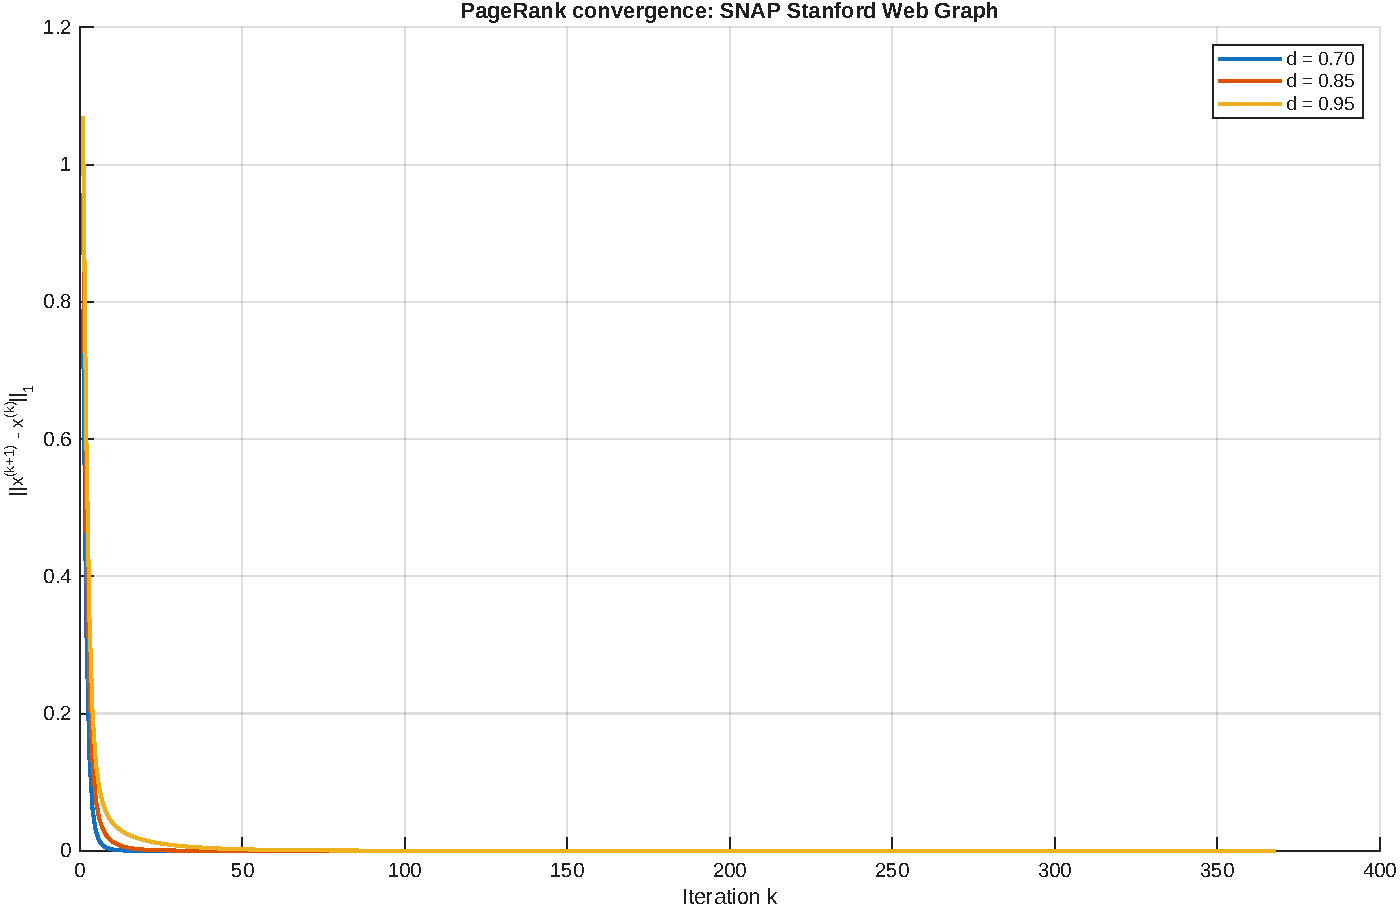
\includegraphics[
width=0.90\textwidth
]{pagerank_convergence.pdf}
\caption{
Convergence of PageRank power iteration
for three damping factors.
The plotted quantity is the
$L^1$ difference between
successive iterates.
}
\label{fig:pagerank_convergence_matlab}
\end{figure}

\subsection{Numerical Verification}

Our implementation also verifies
that the computed PageRank
vectors satisfy the expected
probability constraints.

For all three damping factors,

\[
\sum_{i=1}^{n}r_i\approx1.
\]

The smallest computed
components were

\[
\begin{aligned}
d=0.70:\quad&
\min_i r_i
=1.065366\times10^{-6},\\
d=0.85:\quad&
\min_i r_i
=5.333686\times10^{-7},\\
d=0.95:\quad&
\min_i r_i
=1.784917\times10^{-7}.
\end{aligned}
\]

Every computed component
was therefore strictly positive.

The fixed-point residuals
were also below $10^{-10}$.

These observations are
consistent with the
mathematical properties
established by the
Perron--Frobenius theorem.

In particular, the Google
matrix possesses a unique
strictly positive stationary
probability distribution,
and the numerical iteration
converges toward it.

\subsection{Ranking the Web Pages}

We now examine the
PageRank scores computed
using the damping factor

\[
d=0.85.
\]

The highest-ranking node
has SNAP identifier

\[
89073
\]

and PageRank score

\[
r_{89073}\approx0.011303.
\]

The second and third
highest-ranking nodes have
scores approximately

\[
0.009268
\quad\text{and}\quad
0.008297,
\]

respectively.

The fourth highest score
is approximately

\[
0.003023.
\]

Thus, the first three
nodes receive substantially
higher stationary
probabilities than
the remaining nodes
in the top-twenty ranking.

Figure~\ref{fig:pagerank_top20_matlab}
displays the twenty largest
PageRank scores.

\begin{figure}[htbp]
\centering
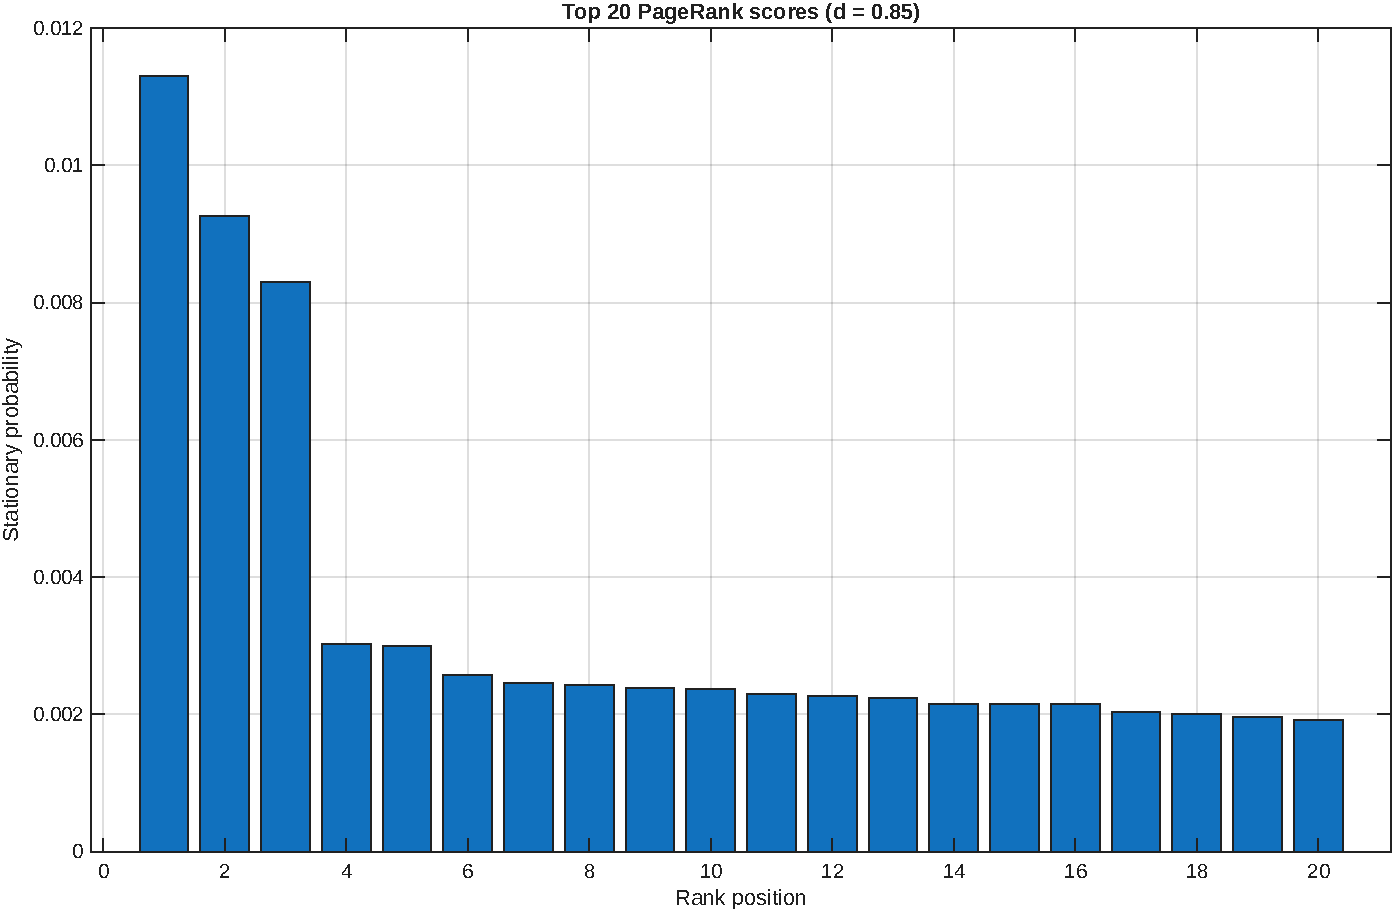
\includegraphics[
width=0.90\textwidth
]{pagerank_top20.pdf}
\caption{
The twenty largest PageRank scores
for the Stanford Web Graph
with damping factor $d=0.85$.
The horizontal axis indicates
ranking position, with position
one corresponding to the
highest-scoring node.
}
\label{fig:pagerank_top20_matlab}
\end{figure}

These scores can be interpreted
as stationary probabilities
in the modified random-surfer
model.

For example, the highest-ranking
node receives approximately
$1.13\%$ of the total
stationary probability.

Although the graph contains
more than $280{,}000$ nodes,
the stationary distribution
is not uniform.

Instead, it reflects
the hyperlink structure
together with the
teleportation mechanism.

\subsection{Computational Discussion}

The experiment demonstrates
the practical importance
of sparse matrix methods.

A dense matrix containing
$n^2$ double-precision
entries would require

\[
8n^2\text{ bytes}
\]

of memory.

For $n=281{,}903$,
this corresponds to
approximately

\[
636\text{ GB}
\]

of storage in decimal units.

Such a representation
would be unnecessarily
expensive for this dataset.

Our implementation instead
stores only the nonzero
entries of the weighted
linking matrix and handles
teleportation implicitly.

As a result, all three
PageRank experiments
completed in a few seconds
on the test machine.

The runtimes reported here
are measurements from
this particular MATLAB
execution and should not
be interpreted as
hardware-independent
performance guarantees.

The numerical experiment
also illustrates an
important tradeoff.

A larger damping factor
places greater emphasis
on the original hyperlink
structure, but may require
more iterations for convergence.

A smaller damping factor
increases the contribution
of teleportation and
provides a stronger
worst-case contraction bound.

Thus, the damping parameter
affects both the mathematical
model and its computational
behavior.

Overall, our experiments
confirm that PageRank can
be computed efficiently
on large sparse directed
graphs using power iteration,
while retaining the
existence, uniqueness,
and convergence guarantees
developed earlier in
this note.



\section{Conclusion}

In this note, we have explored the
Perron--Frobenius theorem, beginning with
the elementary properties of positive
matrices and gradually developing its
connections to stochastic matrices,
Markov chains, and Google's PageRank
algorithm.

Our mathematical investigation began
with the question of whether a matrix
whose entries are strictly positive
must possess a positive eigenvalue
with a corresponding strictly positive
eigenvector.

By constructing an optimization problem
over the standard simplex and using
compactness, we established the existence
of such an eigenvalue and eigenvector.

We subsequently proved that this
eigenvalue is equal to the spectral radius,
is algebraically simple, and strictly
dominates every other eigenvalue
in absolute value.

These properties distinguish positive
matrices from arbitrary square matrices
and provide the foundation for many
important results in matrix theory.

We then introduced stochastic matrices
and showed how their eigenvectors
corresponding to the eigenvalue one
describe stationary probability
distributions.

This connection allowed us to interpret
the evolution of a Markov chain through
repeated matrix multiplication.

In particular, we saw that the
Perron--Frobenius theorem provides
sufficient conditions for the existence
of a unique positive stationary
distribution and convergence toward it.

The mathematical framework was then
applied to Google's PageRank algorithm.

By representing hyperlinks as a directed
graph and constructing a weighted
transition matrix, we demonstrated
that the problem of ranking web pages
can be formulated as an eigenvalue
problem.

We also explained how dangling pages,
teleportation, and the damping factor
modify the transition matrix to obtain
desirable mathematical properties.

The resulting PageRank vector satisfies

\[
Gr=r,
\qquad
r>0,
\qquad
\mathbf{1}^Tr=1.
\]

Our numerical implementation in MATLAB
used the Stanford Web Graph dataset,
containing $281{,}903$ nodes and
$2{,}312{,}497$ directed edges.

The experiments demonstrated that
PageRank can be computed efficiently
using sparse matrix operations and
power iteration.

We also observed that the damping
factor has a substantial influence
on the convergence rate, in agreement
with our theoretical error estimate

\[
\|x^{(k)}-r\|_1
\leq
d^k\|x^{(0)}-r\|_1.
\]

Beyond these mathematical and
computational results, the history
of the subject is equally fascinating.

The theory originated in the work
of the German mathematicians
Oskar Perron (1880--1975) and
Ferdinand Georg Frobenius (1849--1917).

In 1907, Perron established fundamental
spectral properties of matrices
with strictly positive entries.

Frobenius subsequently developed
the theory further, notably in 1912,
extending important results to
nonnegative matrices.

Their work helped establish a
mathematical framework whose
applications would eventually extend
far beyond the problems that
originally motivated its development.

Another remarkable historical
connection concerns the Russian
mathematician Andrey Markov
(1856--1922).

Markov developed the theory of
dependent random variables while
investigating the extent to which
classical probability results,
including the law of large numbers,
could remain valid without
assuming independence.

In a particularly interesting
application published in 1913,
Markov investigated the arrangement
of vowels and consonants in
Alexander Pushkin's
\emph{Eugene Onegin},
a celebrated Russian novel in verse.

By examining the dependence between
successive letters, he demonstrated
how probabilistic reasoning could
be applied to literary text.

It is a remarkable historical
connection that mathematical ideas
now used in search engines,
communication systems, and data science
were also developed and illustrated
through the statistical analysis
of poetry.

It is equally important to recognize
the limitations of our PageRank model.

Although the original PageRank
method was described in publicly
available research, the complete
ranking algorithms used by Google
today are not publicly disclosed.

Google's modern search systems
consider many additional signals
and have evolved considerably
since the original PageRank model.

Consequently, the algorithm
implemented in this note should
be understood as a mathematical
reconstruction of the classical
PageRank framework, based on its
publicly documented principles.

It is not intended to reproduce
the complete proprietary ranking
system used by Google.

Nevertheless, this simplified
model captures an important
mathematical idea: the significance
of a node in a network can be
determined recursively from
the significance of the
nodes connected to it.

Finally, it is worth emphasizing
that the theory of positive and
nonnegative matrices is far
from a closed chapter of mathematics.

Research in this field continues,
including investigations involving
spectral graph theory, nonnegative
tensors, nonlinear eigenvalue problems,
large-scale numerical computation,
and applications in data science.

The theory is especially fascinating
because seemingly elementary
assumptions about matrix entries
can lead to remarkably strong
conclusions about eigenvalues,
eigenvectors, stability,
and long-term behavior.

What began as a mathematical
investigation into the spectral
properties of special classes
of matrices has developed into
a powerful collection of ideas
with applications across
mathematics and computation.

The Perron--Frobenius theorem
therefore illustrates a broader
lesson in mathematics:
abstract theoretical results,
sometimes developed long before
their practical applications
are imagined, can eventually
become essential tools
for understanding and solving
problems in the modern world.


% ------------------------------------------------
% References
% ------------------------------------------------

\begin{thebibliography}{99}

\bibitem{strang}
Gilbert Strang,
\textit{Linear Algebra and Its Applications},
4th edition,
Brooks/Cole, Cengage Learning, 2006.

\bibitem{schultz}
Andrew Schultz,
\textit{Abstract Linear Algebra},
MATH 416, Spring 2010,
University of Illinois at Urbana--Champaign.



Available at:
\url{https://palmer.wellesley.edu/~aschultz/w10/math416/coursenotes.html}

\bibitem{brinpage}
Sergey Brin and Lawrence Page,
``The Anatomy of a Large-Scale Hypertextual
Web Search Engine,''
\textit{Computer Networks and ISDN Systems},
Vol. 30, Nos. 1--7,
pp. 107--117, 1998.

Available at:
\url{https://research.google/pubs/the-anatomy-of-a-large-scale-hypertextual-web-search-engine/}

\bibitem{snap}
Jure Leskovec and Andrej Krevl,
\textit{SNAP Datasets: Stanford Large
Network Dataset Collection},
Stanford University, 2014.

Stanford Web Graph Dataset.

Available at:
\url{https://snap.stanford.edu/data/web-Stanford.html}

\bibitem{hawkins}
Thomas Hawkins,
``Continued Fractions and the Origins
of the Perron--Frobenius Theorem,''
\textit{Archive for History of Exact Sciences},
Vol. 62,
pp. 655--717, 2008.

DOI:
\url{https://doi.org/10.1007/s00407-008-0026-x}

\bibitem{markov}
Andrey A. Markov,
``An Example of Statistical Investigation
of the Text Eugene Onegin Concerning
the Connection of Samples in Chains,''
1913.

English translation published in
\textit{Science in Context},
Vol. 19, No. 4,
pp. 591--600, 2006.

DOI:
\url{https://doi.org/10.1017/S0269889706001074}

\end{thebibliography}
\end{document}